\documentclass[../ClassicThesis.tex]{subfiles}
\begin{document}
%************************************************
\chapter{Adjacency Plategraph / Klara}\label{ch:graph}
\newcommand{\TODO}[1]{\textcolor{red}{\\ \textbf{TODO:} #1 \\}}
%************************************************


% Use active Voice (we do….)
% Ein Gedanke pro Paragraph
% Terminologie anpassen über alle Arbeiten hinweg (was ist eine Plate für alle…)
% Jeder sollte eine kleine Related Work section haben
% Erklärungen zu warum dieser Algorithmus genutzt wurde und nicht ein anderer + limitations des gewählten Algorithmus
% Hübsche Bildchen zum anschaulichen Erklären!! (ebenfalls konsistent halten: gleich geformte labels etc.)
% FROM SOLUTION TO PROBLEM /DISCUSSION
% EXPLAIN ALL VARIABLES ETC.!!!

% 1. Was macht es inhaltlich
% 2. Was kann/tut der Graph überhaupt?


% \paragraph{Why is this part necessary?}
On the basis of the plategraph we can create connectors for plates in the later step \hyperref[ch:joints]{joint creation}. Depending on angles and neighborhood relationships an adequate connector type can be chosen.
% for what? to figure out joint connections?

% \paragraph{What is being achieved in this Chapter?}
In this step we analyse the spatial arrangement of plate objects in 3D-space to create a graph structure which tracks the adjacency. The plates to be analysed are found in the previous step \hyperref[ch:plates]{Plates}. Two or more plates are adjacent to another when at least one side touches or overlaps with the other plate. In addition, the angles in between the plates are calculated.
% WHAT IS WITH THE 3D SNIPPETS??? DO THEY STILL EXIST?

\begin{figure}[!ht]
\centering
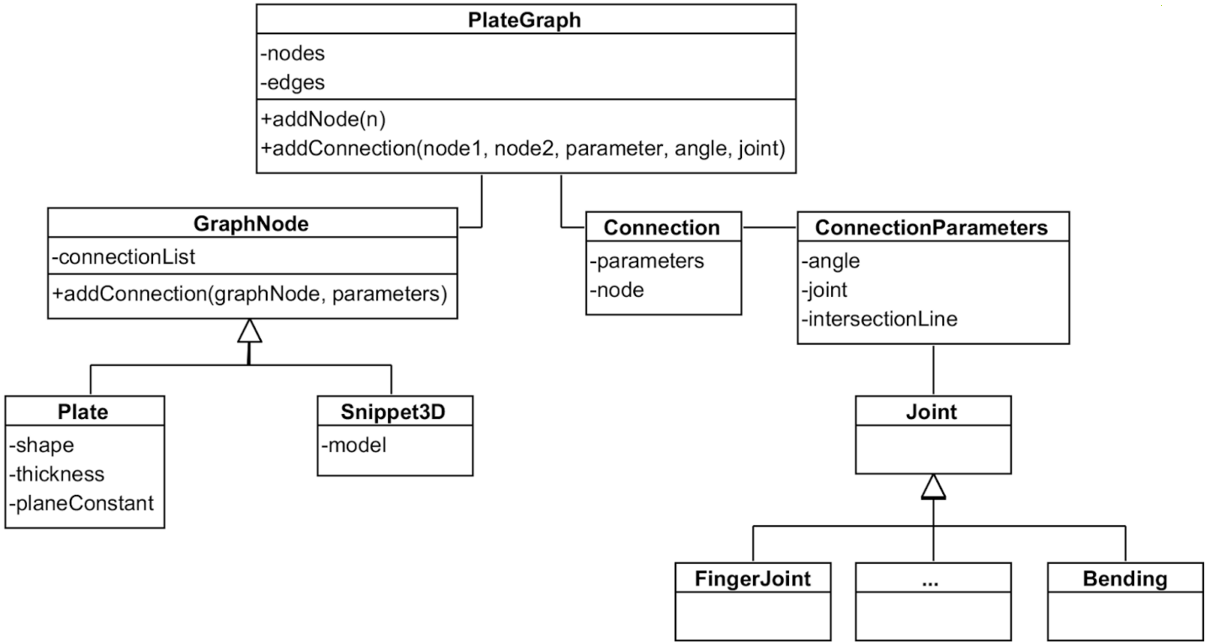
\includegraphics[width=1\columnwidth]{Images/GraphStructure.png}
\caption{Class diagram of the plategraph structure. Nodes and Connections can be added to the graph when a new intersection has been found.}
\label{fig:graphClassDiagram}
\end{figure}
% \paragraph{Chosen Graph Class Structure}
The graph, shown in figure \ref{fig:graphClassDiagram}, holds two lists. One tracks the parts which have been found by the previous step \hyperref[ch:plates]{Plates}. Such a part is called graph node. And the other list tracks the connections of the nodes which we call edge. \\
Each node saves all edges it belongs to in a connection list. Each connection exists twice, one for each node it connects. Therefore we can traverse from one node to another via such a connection. Additionally, a connection saves properties like the angle and the intersection line at which the current node will need to add its joints in the next \hyperref[ch:joints]{step}. Which type of joint is created there depends on the type which is saved in the connections property \emph{joint}.\\
The parts which can be connected are plates. But we support the existence of other node types such as a 3D-snippet which is a part of the model which has not been converted to plates.

\section{Detecting spatial arrangement}
% \subparagraph{requirements for running the algorithm}
% unnecessary??
As a prerequisite the step \hyperref[ch:plates]{Plates} needs to find inherent or create extruded plates first. Afterwards the plane-plane intersections of all combinations of both sides of the plates are computed which results in up to four intersection lines. In preparation for the joint generation step \ref{ch:joints} we truncate the inner intersection lines which would otherwise overlap with adjacent plate intersections.

\subsection{Finding intersections}\label{findIntersections}
% \subparagraph{concrete explanation, functions used/example code etc.}
When two planes intersect there is an intersection line. Since we work with plates which equal two parallel planes we expect to find up to four intersection lines.\\
First, we retrieve the direction vector \emph{dir} of an intersection line between two plates by calculating the cross vector of both normals. In order to retrieve all possible intersection lines of two plates we then calculate four possible plane-plane intersections of 
\begin{itemize}
\item the two main sides of the plates
\item the two parallel sides of the plates
\item one main and one parallel side 
\item one parallel side and one main side
\end{itemize}
\*\\
First, a possible position vector \emph{p} has to be found which lies on both planes \cite{positionVectorRetrieval}.
\\\*\\
\emph{Plane constants:} $d_1, d_2$\\
\emph{Normals:} $\vec{n_1}, \vec{n_2}$
$$ p = \frac{d_1 * \vec{n_{2}}^{2} - d_2 * (\vec{n_1} * \vec{n_2})}{\vec{n_{1}}^{2} * \vec{n_{2}}^{2} - (\vec{n_1} * \vec{n_2})^{2}} * \vec{n_1} + \frac{d_2*\vec{n_1}^2 - d_1*(\vec{n_1} * \vec{n_2})}{\vec{n_1}^2 * \vec{n_2}^2 - (\vec{n_1} * \vec{n_2})^2} * \vec{n_2} $$

On the basis of a position vector \emph{p} and the direction $\vec{dir}$ an intersection line can be computed: $ line = p*x + \vec{dir}$
\\
Now that all lines are found we have to test if the lines actually go through both plates and not only the according planes and that the plates touch. Figure \ref{fig:infiniteIntersections} shows all infinite intersection lines and has the actual plate intersections highlighted.
\begin{figure}[!ht]
\centering
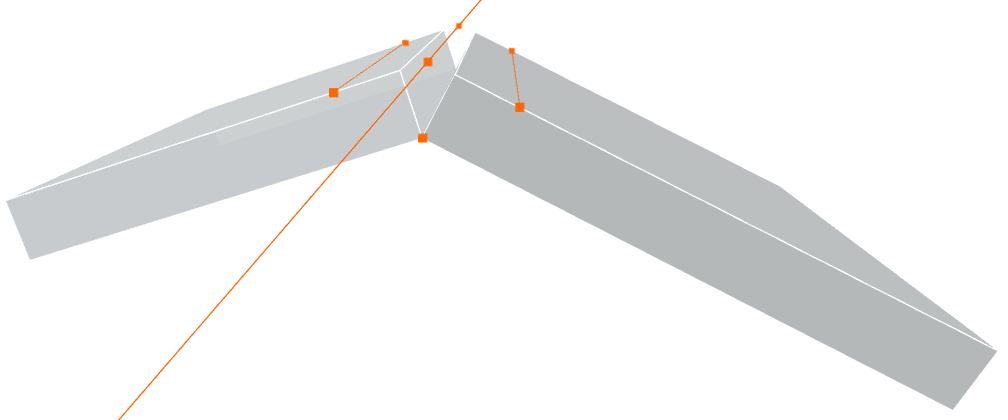
\includegraphics[width=1\columnwidth]{Images/06-1-graph-fourIntersectionLines.png}
\caption{Single plate pair with all of its intersection lines. The infinite line has been clipped to the length of the other lines.}
\label{fig:infiniteIntersections}
\end{figure}
In addition, this step retrieves the exact start and end points of the line segment that defines the intersection of both plates. In order to find these boundaries we calculate the intersections of the lines with all boundary edges of the plates. The result is shown in figure \ref{fig:allBoundaries}.\\
\begin{figure}[!ht]
\centering
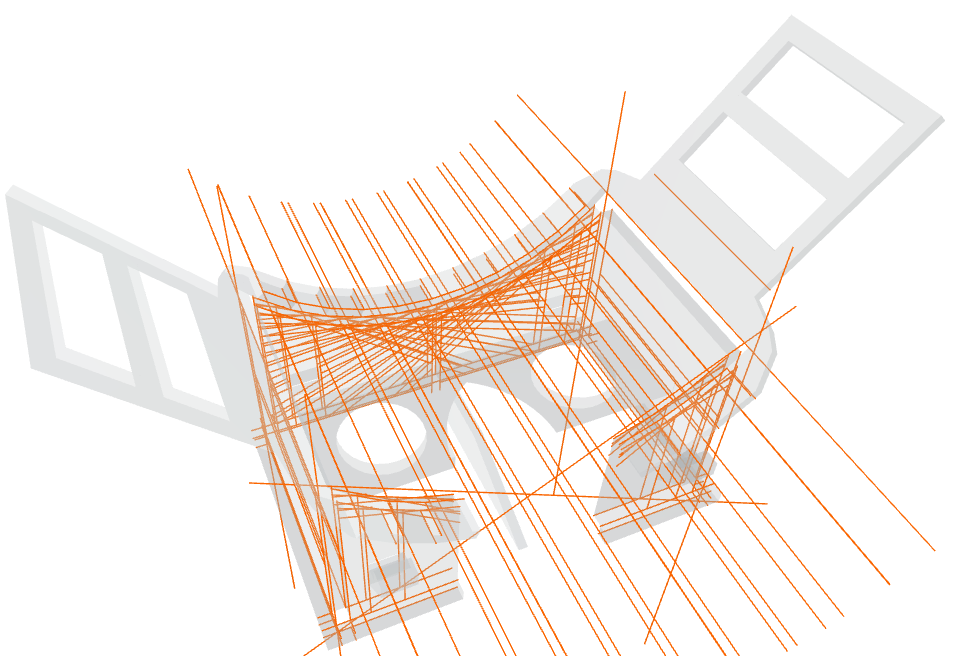
\includegraphics[width=\columnwidth]{Images/AllIntersectionsHMD.png}
\caption{All intersections that were found. }
\label{fig:allBoundaries}
\end{figure}

\section{Preparing plates for connectors}
\subsection{Volume based clipping}
Before joints can be added to the plates we have to prepare them. We cut the shapes back so that the joints do not overlap with the other plate.\\
As seen before, up to four intersectionlines have been calculated per intersection. Two of them lie both on one side of the plate and the other two belong to the second side. The two lines on one side build a rectangle when their ends are connected, see fig. \ref{fig:clippingPlate}. We use those two rectangles to remove the parts of the plates where we will place fingerjoints. The shape is rotated in the xy-plane, as well as the rectangles. A 2-dimensional clipping algorithm is now used to create the new shape. When the shape is rotated back into the 3D-scene, see fig. \ref{fig:3dPlaneClipping}, the overlapping parts of the plates are removed.
\begin{figure}[!ht]
\centering
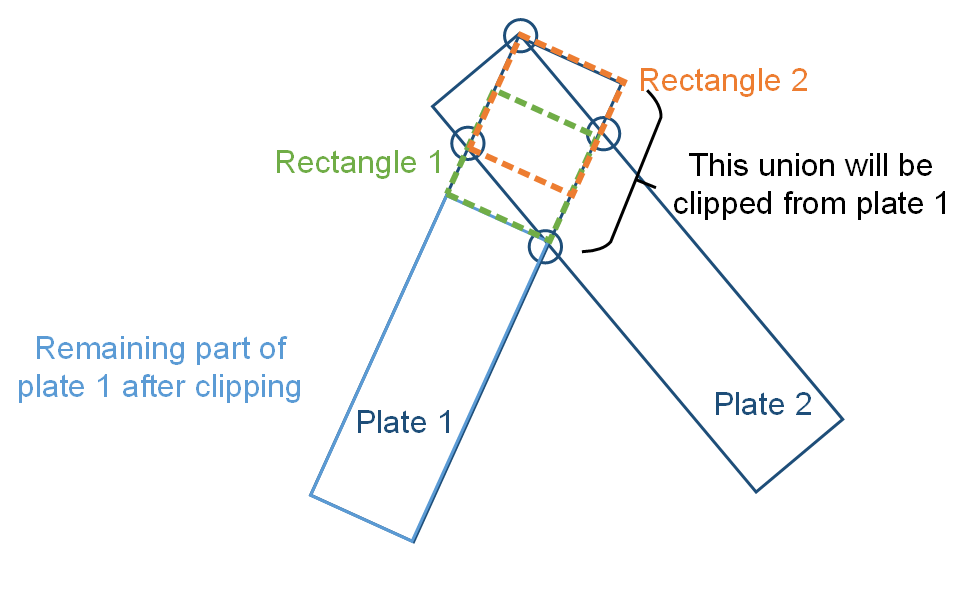
\includegraphics[width=\columnwidth]{Images/10-joints-clippingPlate.png}
\caption{Side view of a single plate pair. The circles mark where there are intersection lines. The rectangles show what is clipped away from plate 1. }
\label{fig:clippingPlate}
\end{figure}

There are cases when not all four lines are actually a plate intersection but only a plane intersection, those cases are shown in fig. \ref{fig:casesOfLines}. 
\begin{figure}[!ht]
\centering
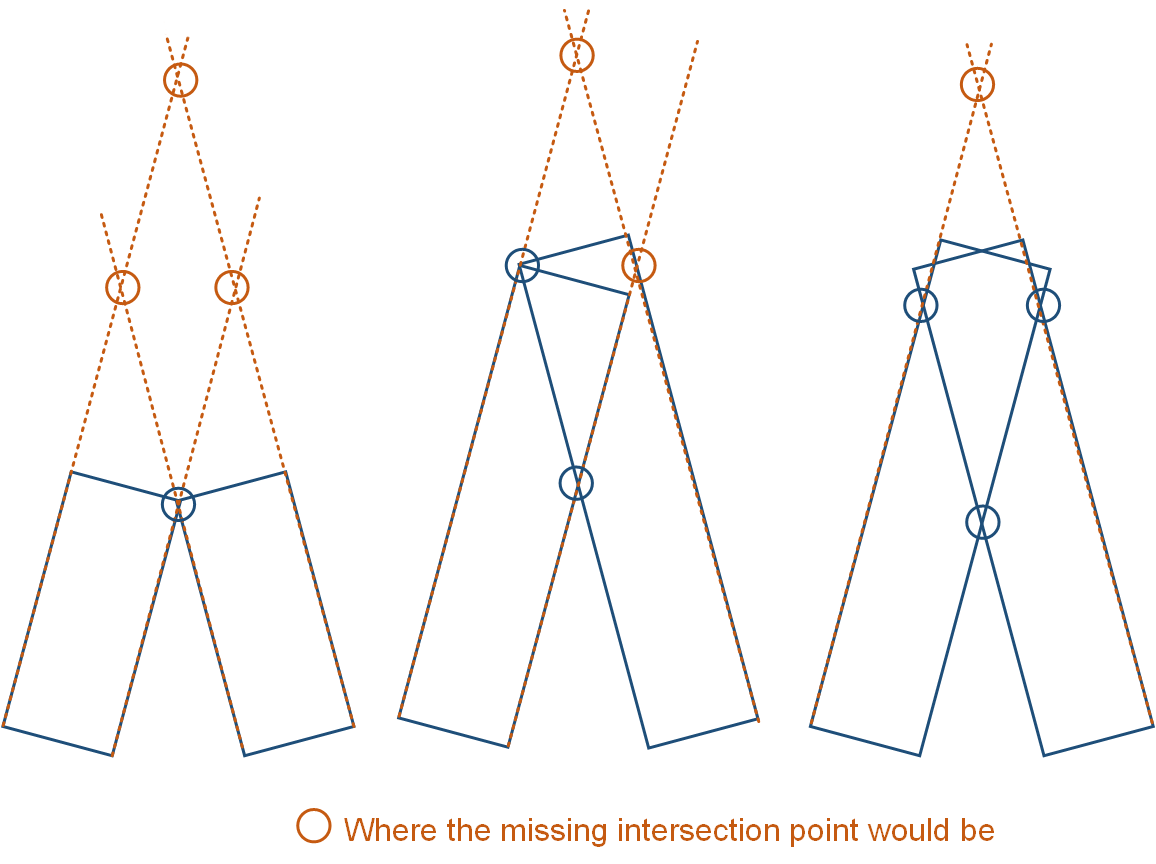
\includegraphics[width=\columnwidth]{Images/10-joints-casesOfLines.png}
\caption{There can also be less than 4 actual intersections. In this case we have to calculate the projected intersection lines as well as the ones which are only a correct plane-plane-intersection but not actually going through a part where the plates overlap}
\label{fig:casesOfLines}
\end{figure}

In such cases the infinitely long plane intersection line will be clipped to match the length of the existing plate intersections. This yields two rectangles as well, which can then be used for clipping the shapes of the plates.
% \begin{figure}[p!]
% \centering
% 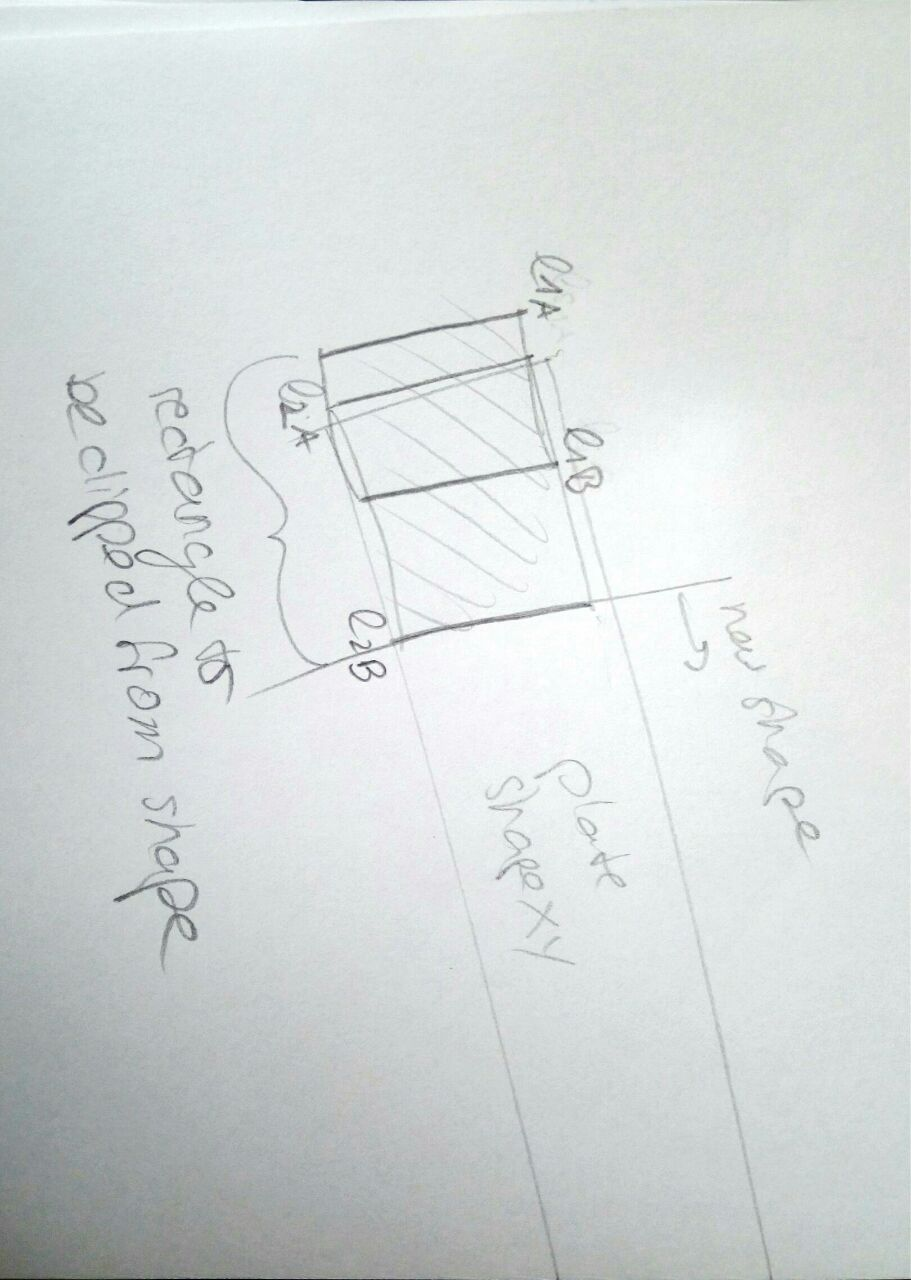
\includegraphics[width=.5\columnwidth, angle=90]{Images/06-1-graph-clippingRectangles.jpg}
% \caption{The shape of the plate is rotated so it lies on the xy-plane. The rectangles derived from the intersection line segments define what has to be clipped away from the shape.}
% \label{fig:planeClipping}
% \end{figure}

\begin{figure}[ht]
    \centering
    \begin{subfigure}[b]{0.45\textwidth}
        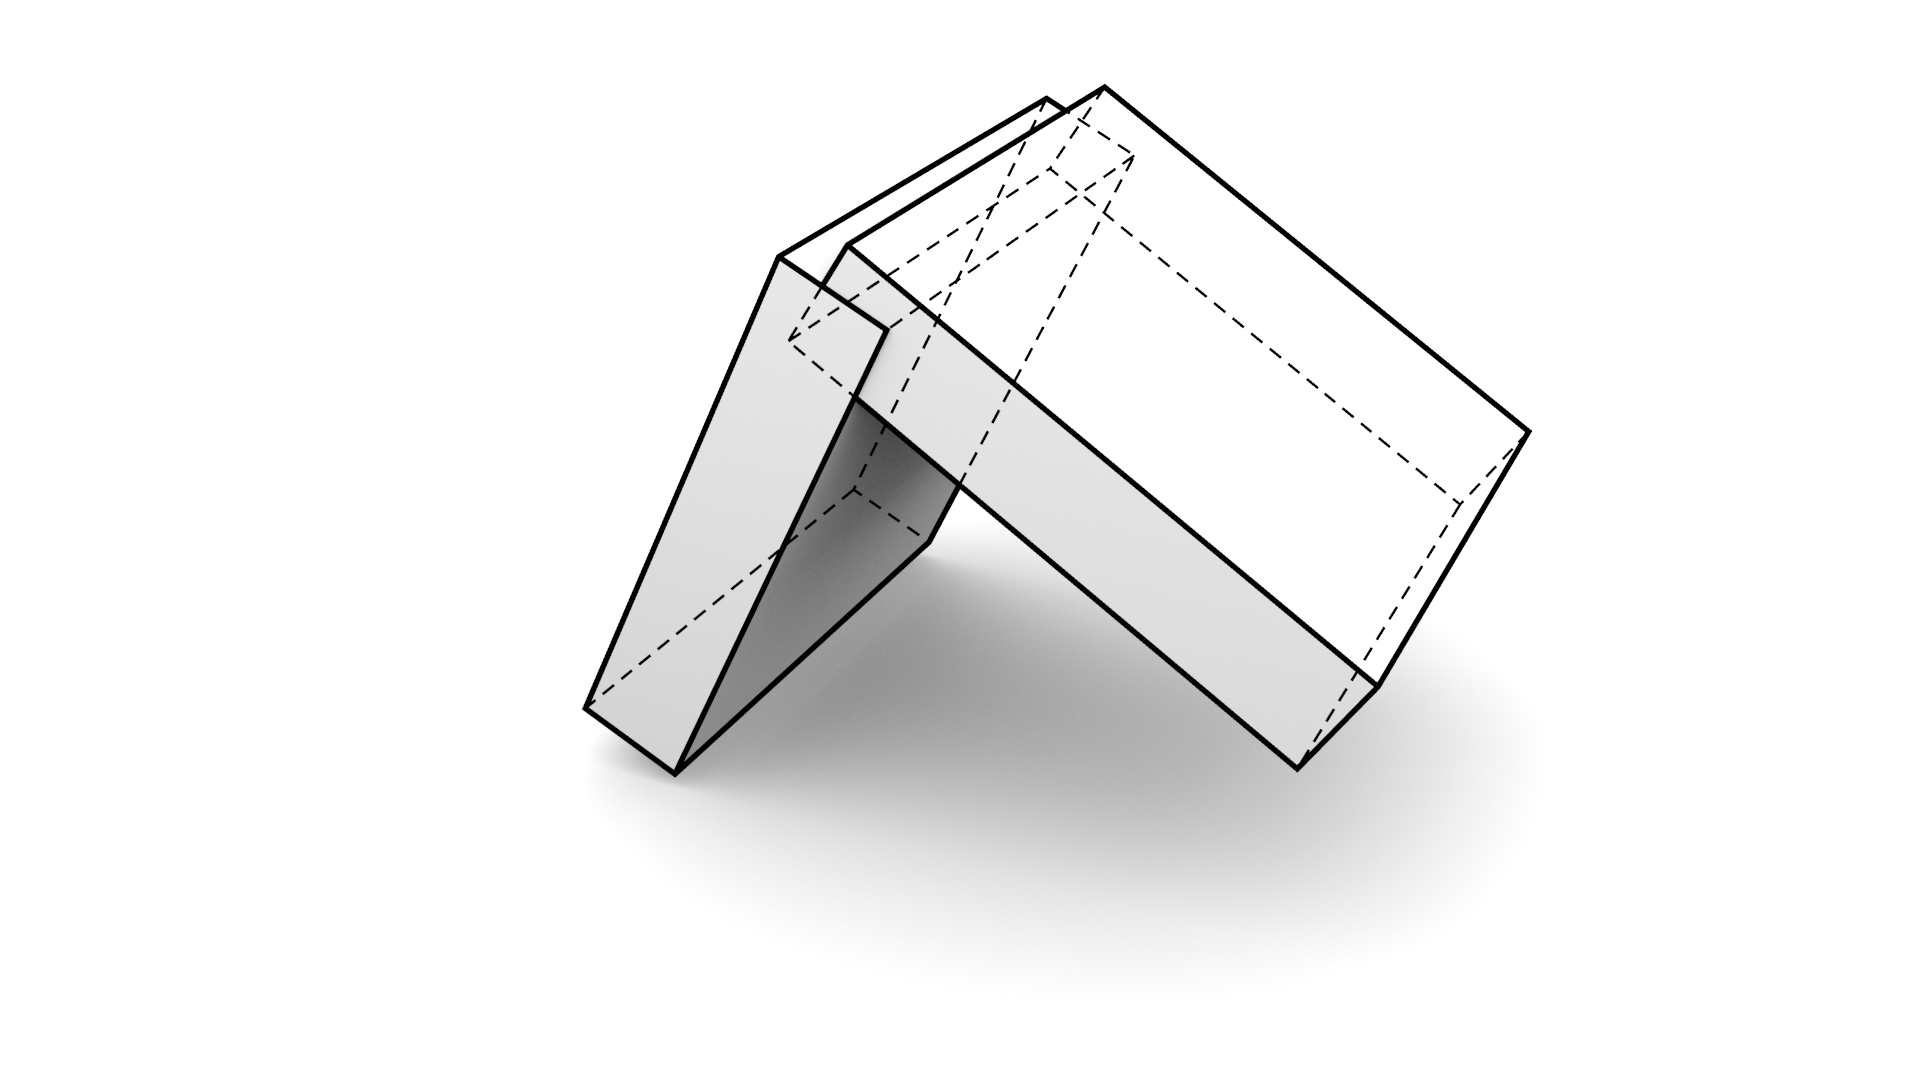
\includegraphics[width=\columnwidth]{Images/BlocksIntersecting.png}
        \caption{Two plates before clipping.}
    \end{subfigure}
    ~
    \begin{subfigure}[b]{0.45\textwidth}
        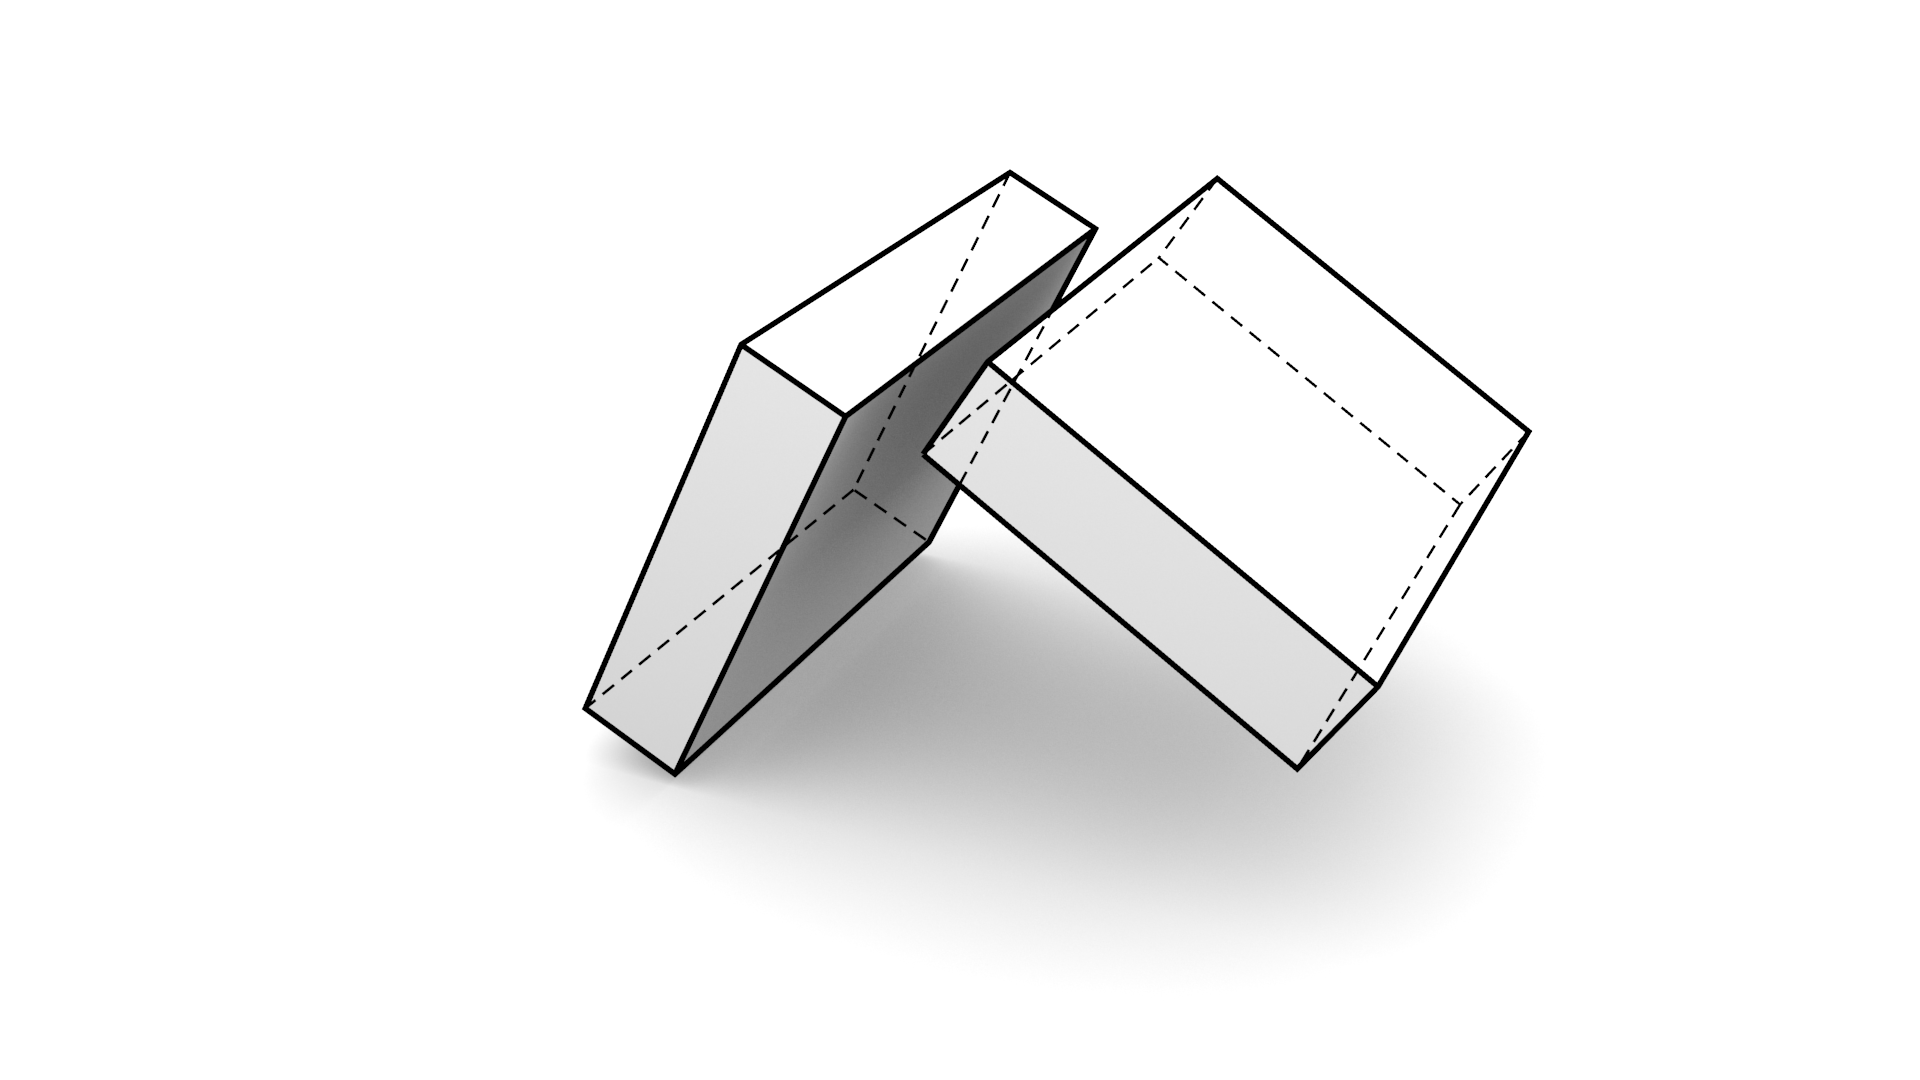
\includegraphics[width=\columnwidth]{Images/BlocksIntersectingshortened.png}
        \caption{Two plates after clipping.}
    \end{subfigure}
    \caption{When the shapes have been cut in 2D they are rotated back to form a 3-dimensional plate again. This figure depicts the volume which was cut off by the algorithm leaving the remaining plates p$_1$ and p$_2$}
    \label{fig:3dPlaneClipping}
\end{figure}


\section{Analyzing spatial arrangement}
\subsection{Angle calculation}\label{angleCalculation}
In order to generate fitting joints in the upcoming step and for grouping plates to bent plates (see Chapter \hyperref[ch:curves]{Curves}) the angles are necessary.\\
First, we determine the angle between the according planes.\\
plane normals: $\vec{u}, \vec{v}$\\
angle between planes: $\theta$
$$ cos(\theta) = \frac{\vec{u} \cdot \vec{v}}{|\vec{u}| * |\vec{v}|}$$
But we are not talking about infinitely large planes instead we want the angle which is enclosed by the finitely large plates. Therefore we need to adjust the angle in some cases.\\
The calculated angle in correct for planes. But depending on where the normals are faced it might be a wrong angle for the plates, see fig. \ref{fig:wrongAngle}, since we need the angle the plates are enclosing.
\begin{figure}[!ht]
\centering
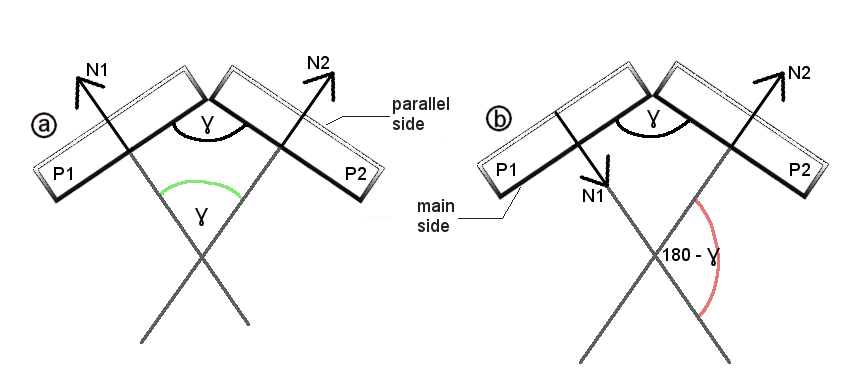
\includegraphics[width= 1\columnwidth]{Images/anglesExamplesSmall.png}
\caption{(a) The angle between the plates' normals correspond with the angle $\gamma$ between the plates. (b) The angle between the plates' normals is in this case an adjacent angle to the requested angle $\gamma$.}
\label{fig:wrongAngle}
\end{figure}
Thanks to the previous clipping step we can find out when the angle has to be adjusted.\\
As can be seen in figure \ref{fig:touchingOrNot}, plates with an acute angle still touch when cut back and plates with an obtuse angle do not.
\begin{figure}[!ht]
\centering
\begin{subfigure}[b]{0.45\textwidth}
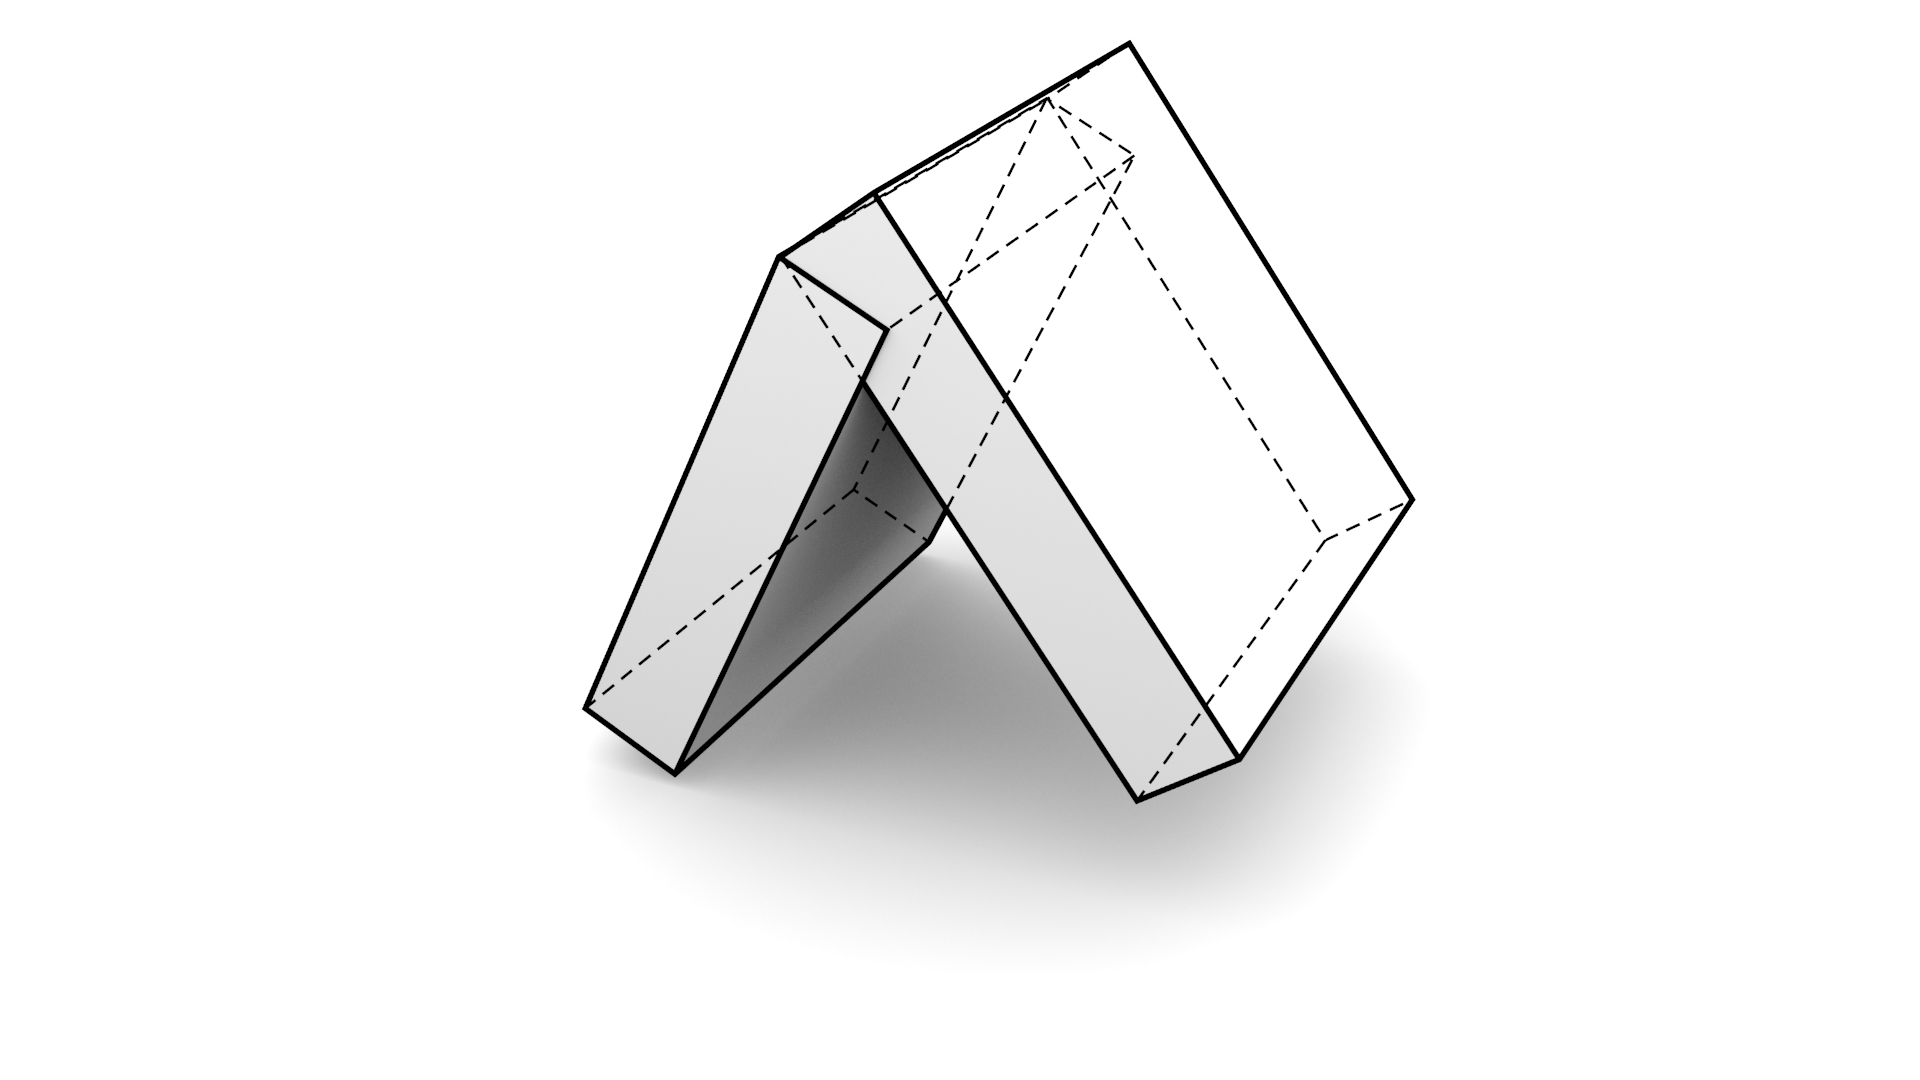
\includegraphics[width=\columnwidth]{Images/Blocks_One_Edge.png}
\caption{Plates with an acute angle.}
\end{subfigure}
~
\begin{subfigure}[b]{0.45\textwidth}
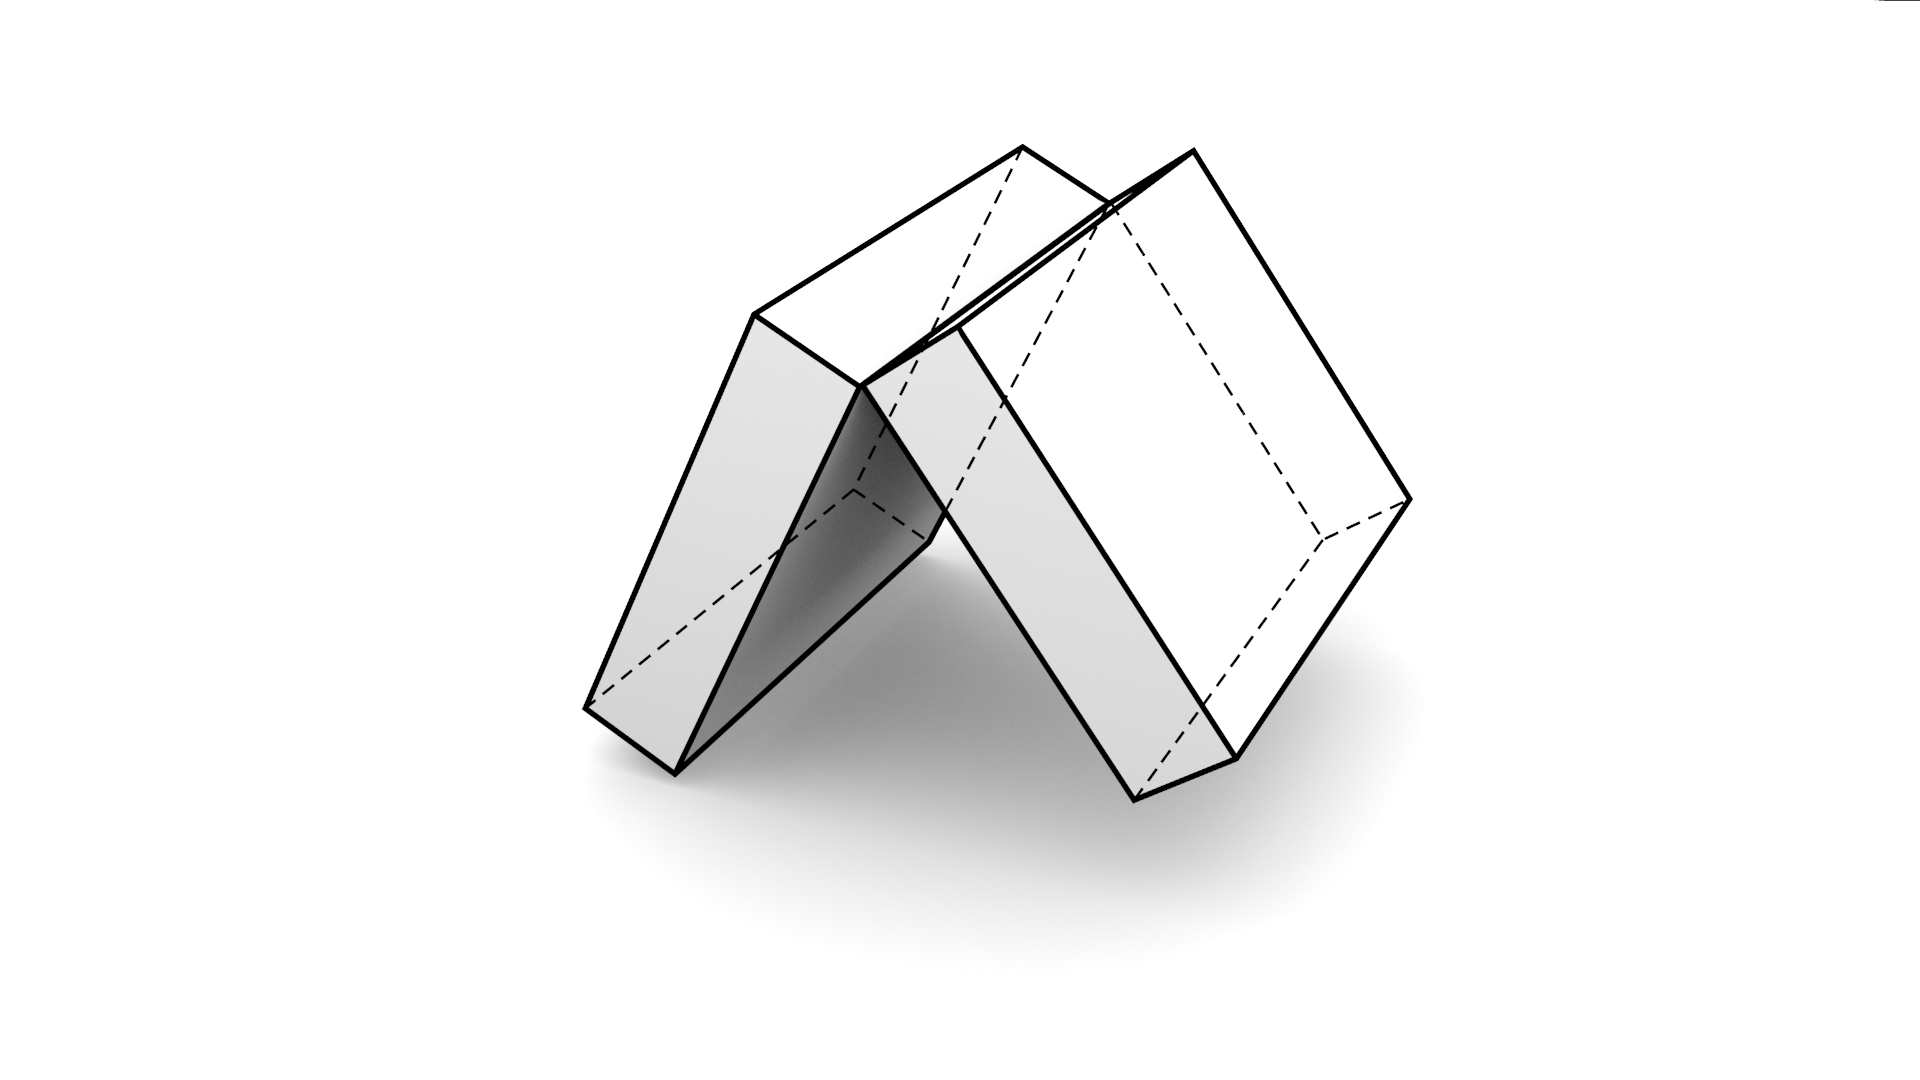
\includegraphics[width=\columnwidth]{Images/Blocks_One_Edge_shortened.png}
\caption{Plates still touch after clipping.}
\end{subfigure}

\begin{subfigure}[b]{0.45\textwidth}
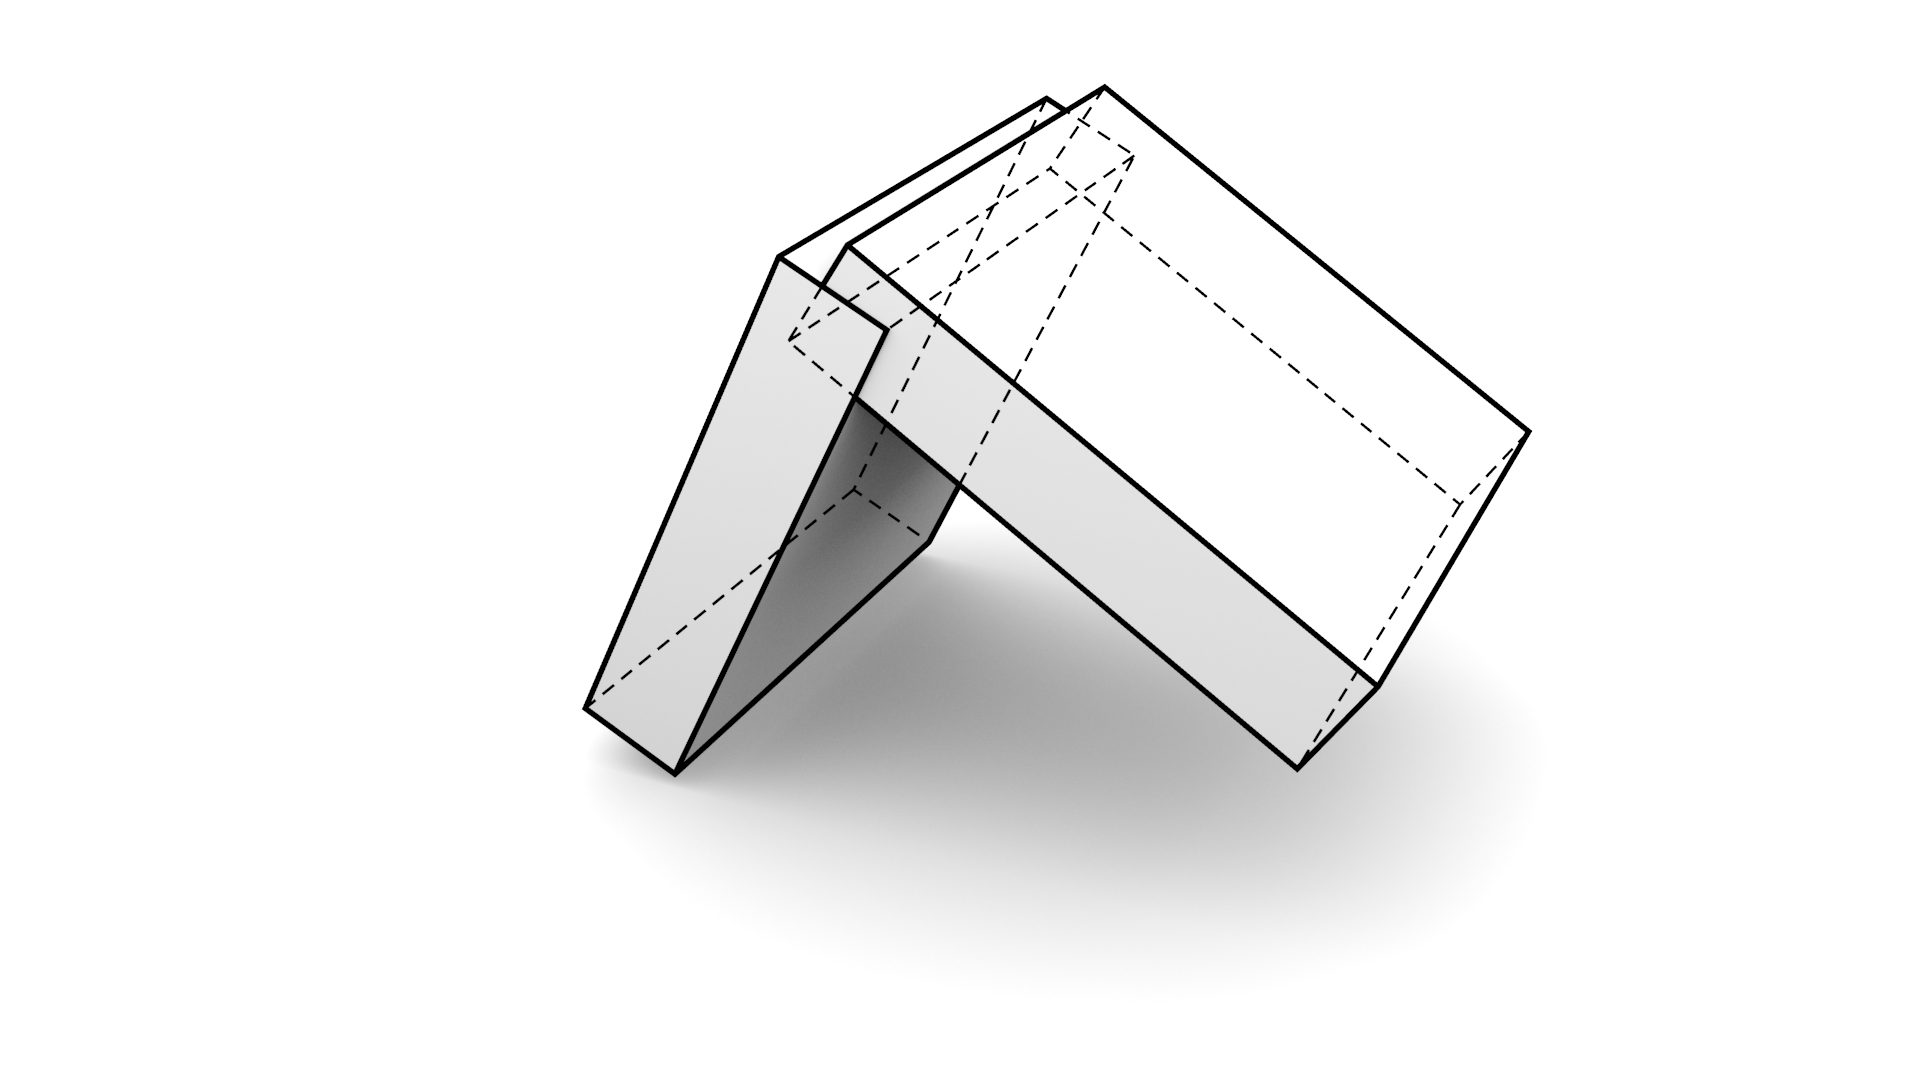
\includegraphics[width=\columnwidth]{Images/Blocks_Intersecting.png}
\caption{Plates with an obtuse angle.}
\end{subfigure}
~
\begin{subfigure}[b]{0.45\textwidth}
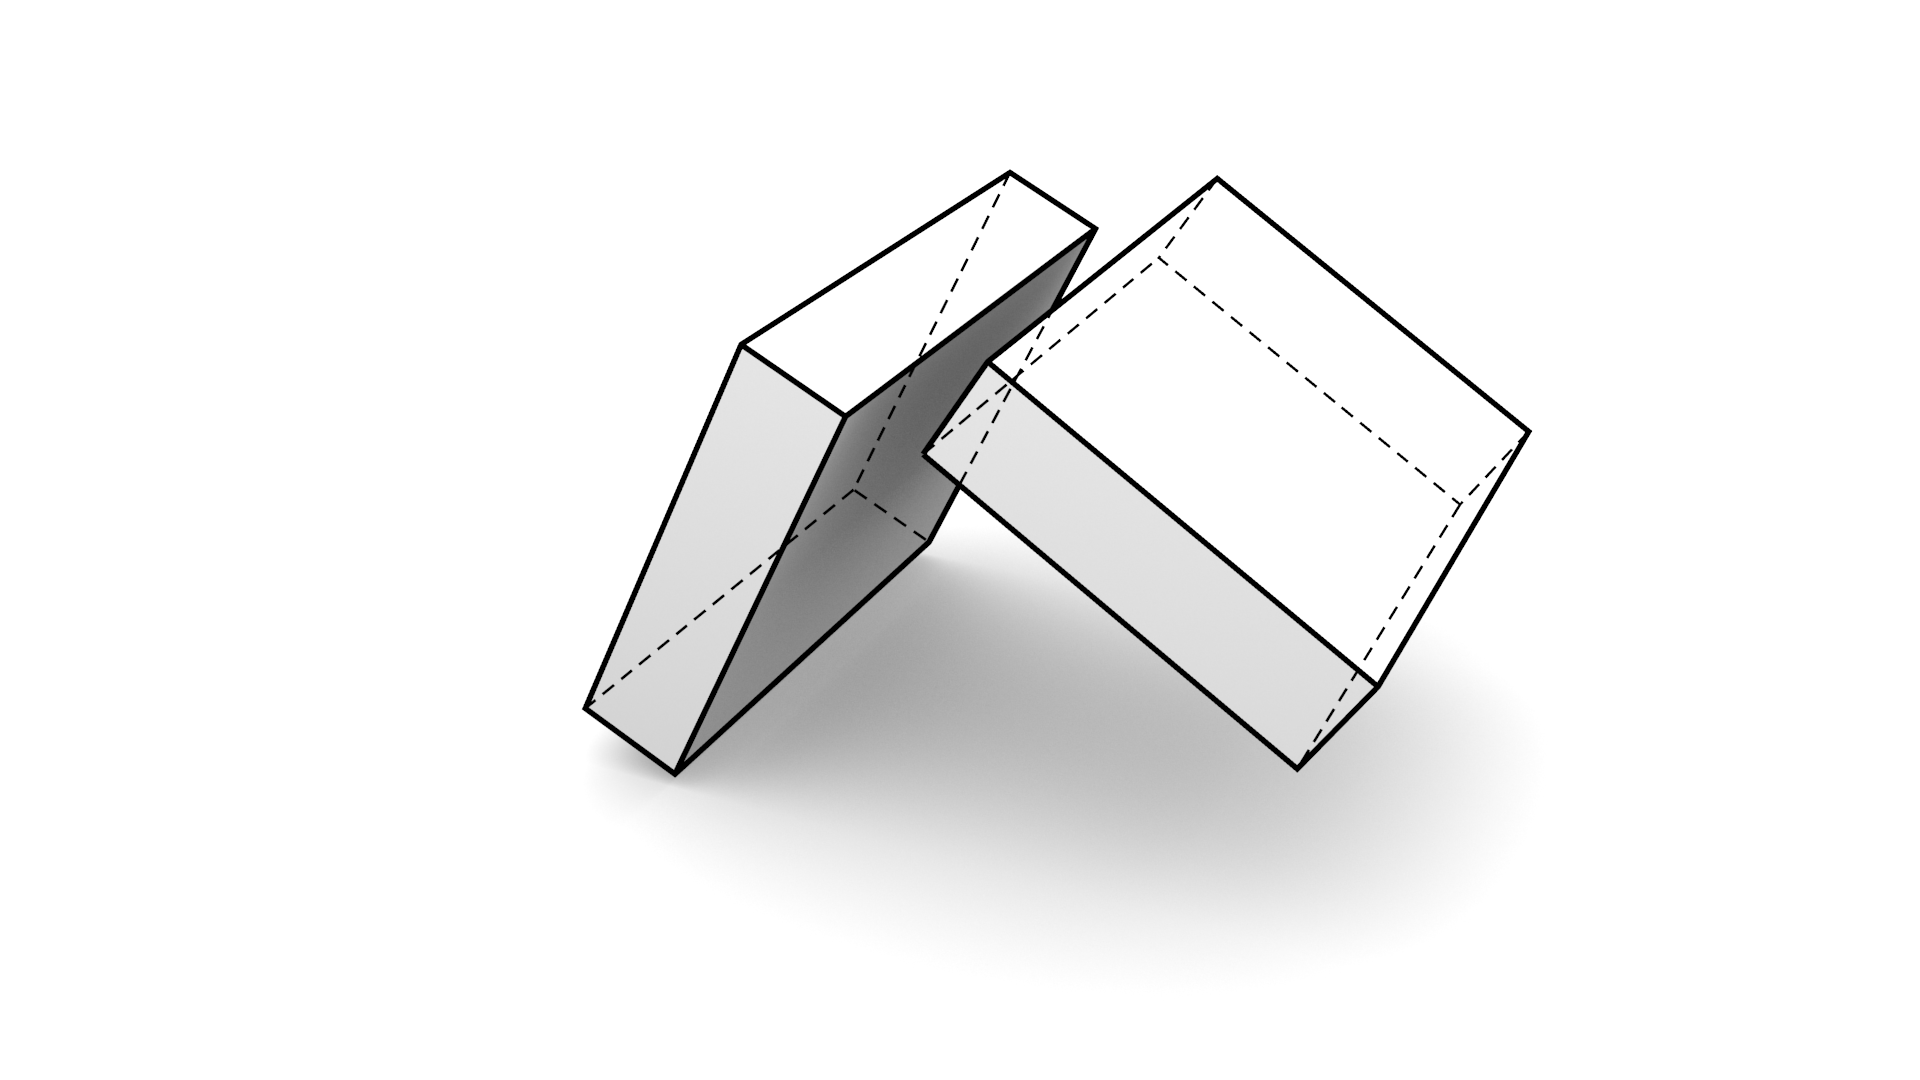
\includegraphics[width=\columnwidth]{Images/Blocks_Intersecting_shortened.png}
\caption{Plates do not touch after clipping anymore.}
\end{subfigure}
\caption{After the clipping process the plate pair might be not touching anymore. This means that the angle between the plates has to be larger than 90$^\circ$.}
\label{fig:touchingOrNot}
\end{figure}

Finally, we test if the plates still touch. This is how we know if the angle should be acute or obtuse. If the originally calculated angle does not correspond with this we adjust the angle by subtracting it from 180$^\circ$.

\subsection{Finding new main lines}\label{mainLine}
In order to know where to add the joints to the plate we have to identify one line segment for each plate whithin a connection.\\
For that we compare the distances of the new edges of the two plates which are shown in figure \ref{fig:mainLinesAfterClipping}. The lines belonging to the smallest distance determine where to place the joints.
\begin{figure}[!ht]
\centering
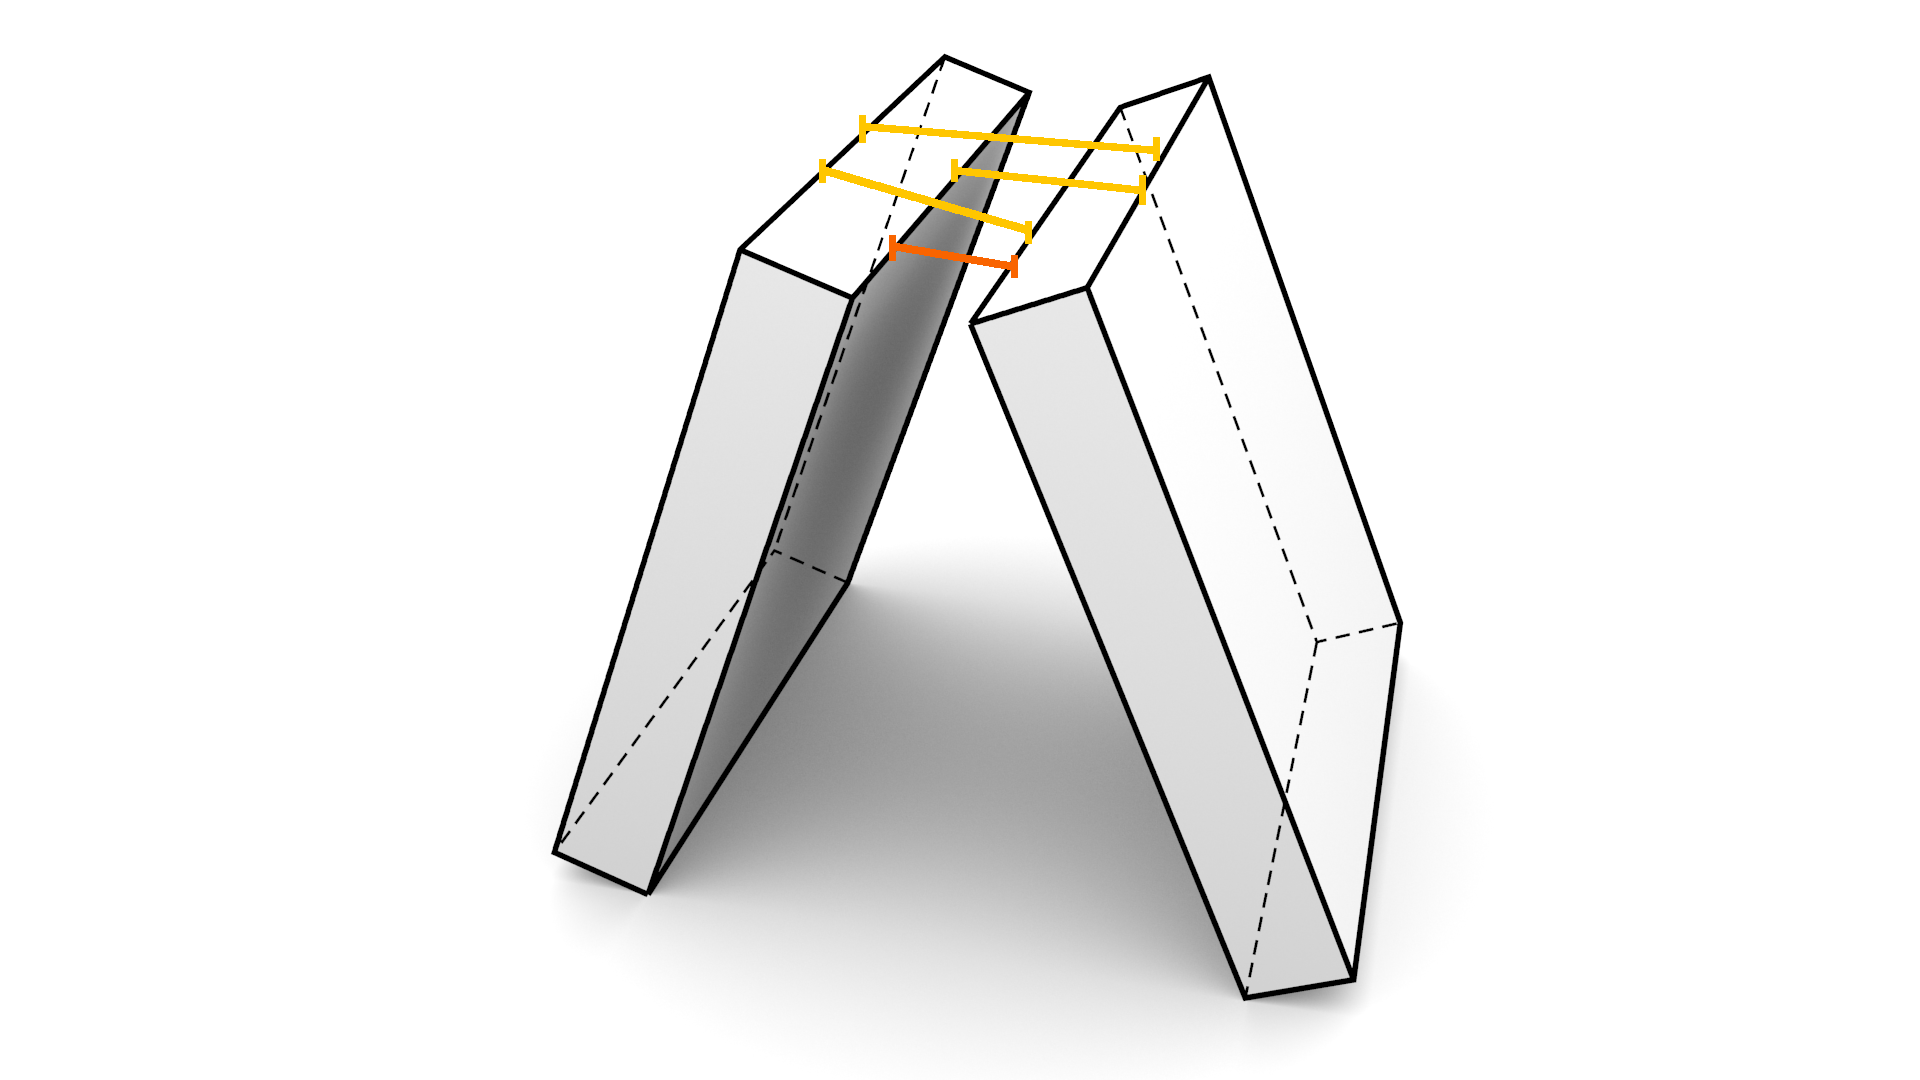
\includegraphics[width=.5\columnwidth]{Images/Blocks_No_Touch.png}
\caption{The distances between the new edges after the clipping process reveals which of them are the inner lines. Those lines will be used for adding joints in the next step.}
\label{fig:mainLinesAfterClipping}
\end{figure}

The segments are called main line for that connection and plate.

\subsection{Truncating intersection lines}
Now that all main lines are known we need to shorten the lines so that no other lines overlap with it. If this step is missing then the following step for creating joints will run in to problems because the joints overlap each other.\\
If we now have a look at only the inner intersections of plates in a model, seen in fig. \ref{fig:innerBoundaries}, we can identify the overlaps.
\begin{figure}[!ht]
\centering
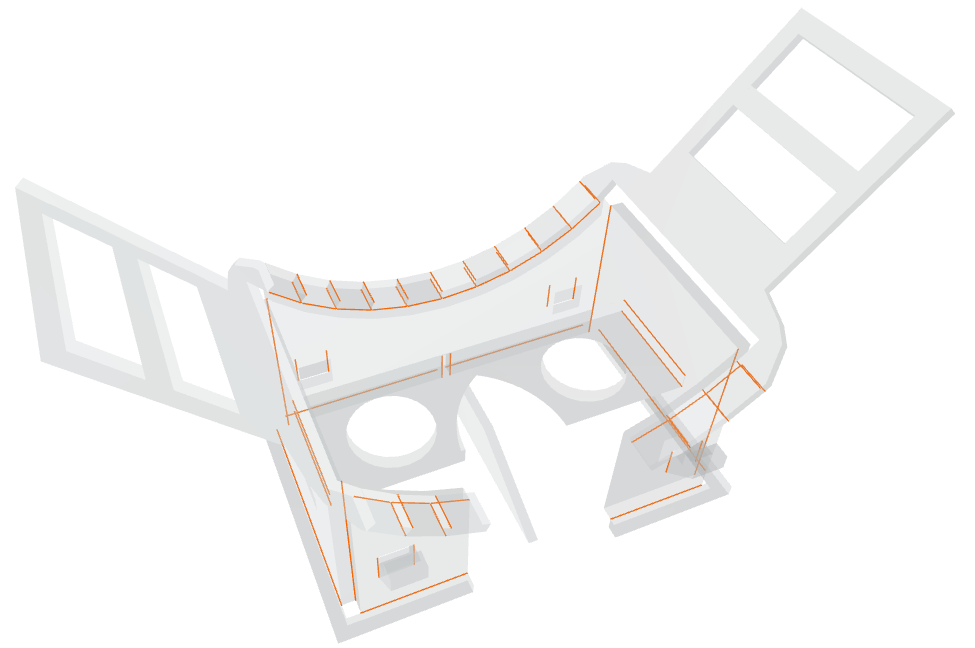
\includegraphics[width=\columnwidth]{Images/TruncatedIntersectionsHMD.png}
\caption{The inner boundaries of the plates overlap. In the next step when joints will be created they are only supposed to be on the inner part of the line. Therefore the lines have to be truncated.}
\label{fig:innerBoundaries}
\end{figure}
For truncating the lines we use the following algorithm \ref{truncateLines}.
\TODO{explain the alogrithm}\\
\begin{algorithm}[H]
	\DontPrintSemicolon
	\KwData{lines}
	\KwResult{truncated lines}
	initialize variables here\;
    \For{line$\_$pair in lines}{
    	line1 = line$\_$pair[0]\;
        line2 = line$\_$pair[1]\;
        point = lineLineIntersection(line1, line2)\;
        \If{isPointOnLine(point, line1) and isPointOnLine(point, line2)}
        {
      		\tcp{linesegments actually cross}
      		startSegmentLine1 = new Line(point, line1.start)\;
            endSegmentLine1 = new Line(point, line1.end)\;
            startSegmentLine2 = new Line(point, line2.start)\;
            endSegmentLine2 = new Line(point, line2.end)\;
            \tcp{the shorter part of each line is discarded}
			\eIf{startSegmentLine1.distance() $>$ endSegmentLine1.distance()}{
				\eIf{startSegmentLine2.distance() $>$ endSegmentLine2.distance()}{
				return \{
                    	endSegmentLine1\;
                        endSegmentLine2
                    \}
				}{
                    return \{
                    	endSegmentLine1\;
                        startSegmentLine2
                    \}
				}
			}{
			return \{
                	startSegmentLine1\;
                    startSegmentLine2
                \}
			}	      
        }
    }
  	\caption{Truncating lines}
  	\label{truncateLines}
\end{algorithm}

Finally, we found all plate adjacencies and necessary information on the connected parts. Also, we adjusted the plates. Therefore the next step explained in Chapter \hyperref[ch:joints]{Joint Creation} can start adding joints.

\section{Alternative approaches}
The solutions presented in this chapter may not be the only way to go. Therefore, we want to give an overview of other algorithms we tried or are aware of and why we replaced them.

\subsection{Possible data structures for intersection tracking}
Dustin Beyer \citeauthor{master-thesis} used an adjacency matrix for keeping track of neighboring plates. All the plates were kept in a plate array. Their indices corresponded to the rows and columns of the matrix. Each cell contained a set of plate adjacency objects. This made it possible that one plate could have more than one connection.\\
\*\\
Instead of an adjacency matrix we used the previously explained plategraph class structure because it allows for traversal along the plates and, additionally, the found edges. \\
Moreover, our structure is open for adding additional objects beside plates. For example 3D-printable snippets which were not converted to plates by our software.

\subsection{Approaches for finding intersections}
In the master thesis on Platener\cite{master-thesis} a connection is calculated by finding all four possible connections between both sides of two plates. Then the edges of the plates are tested against the line. The part of the line overlapping with an edge was kept for further calculations.\\
\*\\
When looking for plate intersections we also calculate all possible intersections. But plates do not always touch each others edges. Therefore we replaced this algorithm by a different approach explained in the previous section for \hyperref[findIntersections]{finding intersections}.

\subsection{Representation of the joint location}
As seen before in the section \hyperref[mainLine]{Main Lines} we calculate one line per intersection and plate which determines where we will place the joints. We chose this approach because it is a straight forward way. The joints only have to be moved onto the line and can directly be added to the plates. \\
A different, more future oriented, approach is to work with the axis going through the middle of where the joints will be. This means it also defines the axis around which the plates could rotate when their angle changes, see both options shown in figure \ref{fig:hinges}. 
\begin{figure}
    \centering
    \begin{subfigure}[b]{0.45\textwidth}
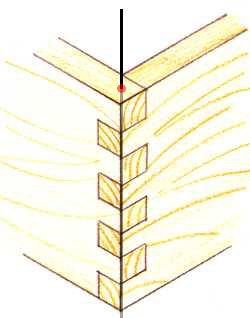
\includegraphics[width=\columnwidth]{Images/woodenFingers.jpg}
\caption{Axis going through the middle of the joints.}
\end{subfigure}
~
\begin{subfigure}[b]{0.45\textwidth}
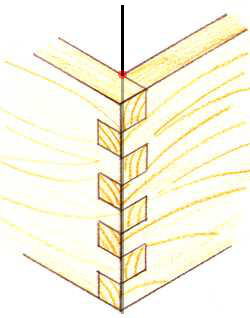
\includegraphics[width=\columnwidth]{Images/woodenFingers2.jpg}
\caption{Plate specific intersection lines}
\end{subfigure}
\caption{Two possible representations of where to place joints.}
    \label{fig:hinges}
\end{figure}
In the case that our software will be extended with an editor the user might want to select an edge and define that the connection should be similar to a hinge. For this you would want rather one axis than two lines specific to a plate. But then the calculation for where to place the joints at the plate becomes more expensive.\\
In our use case the single line approach for an edge of a plate is completely sufficient.

\subsection{Finding main lines by checking if they lie on a corner of the shape}
As already mentioned when plates intersect there can be up to four intersection lines. We need to define which of them is the most important one in order to know where to put joints. The line we wanted to choose had to touch both plates.\\
This means all lines which intersected with any points of the shapes of the plates were ignored. The other line became main line.\\
Our assumption, see fig. \ref{fig:assumption}, which we adopted from the Platener thesis \cite{master-thesis} for finding the main line is the following:\\
Two plates always touch one another edge-to-edge. Therefore, if an intersection line does not lie on an outer boundary of the shape it is the main line.
\begin{figure}[!ht]
\centering
\begin{subfigure}[b]{0.45\textwidth}
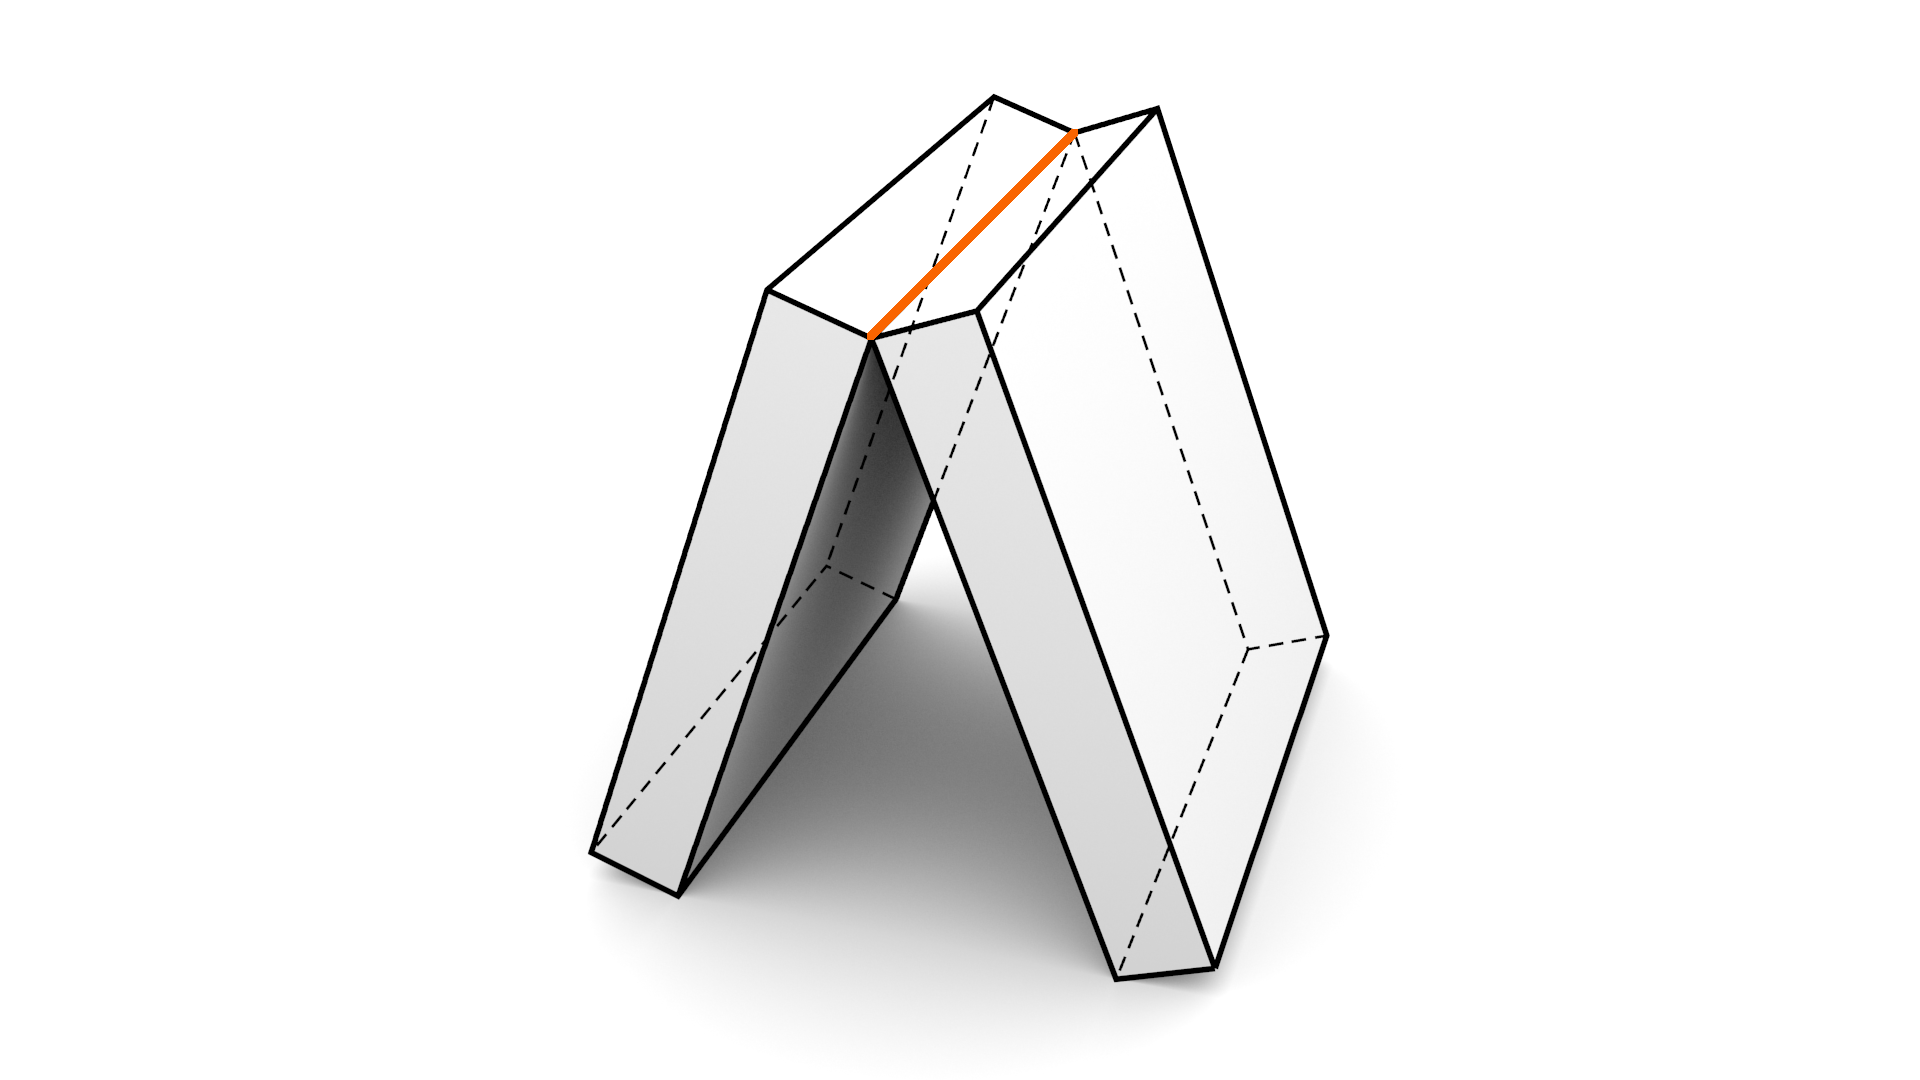
\includegraphics[width=\columnwidth]{Images/1Touching.png}
\caption{The only intersection line was immediately marked as main line.}
\end{subfigure}
~
\begin{subfigure}[b]{0.45\textwidth}
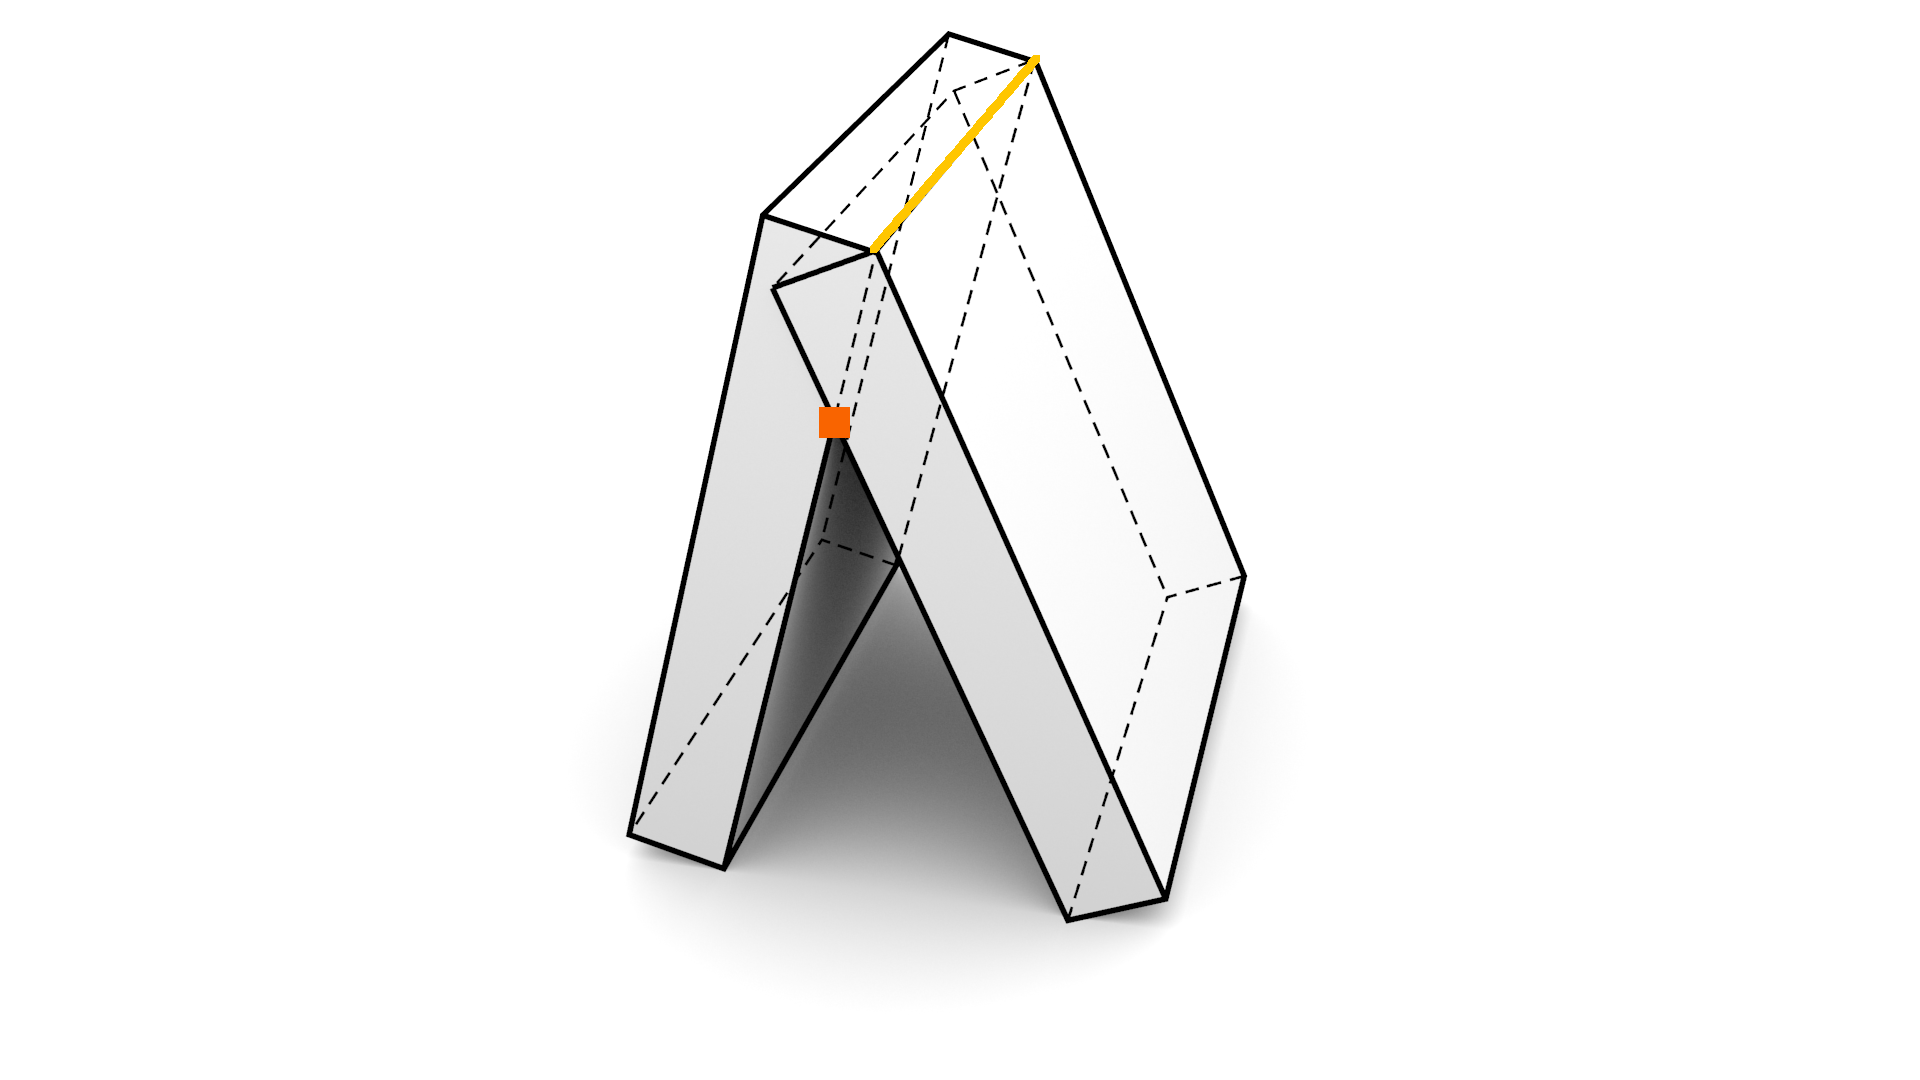
\includegraphics[width=\columnwidth]{Images/2InsideOverlap.png}
\caption{The orange square marks the inner intersection line which we chose as main line.}
\end{subfigure}
\caption{Our assumption was that we only need to define one main line per plate pair. If there was just one intersection at all it was definitely the correct one. And when there were more than one intersection we thought the inner intersection should be the main line. }
\label{fig:assumption}
\end{figure}

But the problem is that plates can intersect in many different ways, see fig. \ref{fig:obtuseAssumption}, which do not all verify our first assumption. 
\begin{figure}[!ht]
\centering
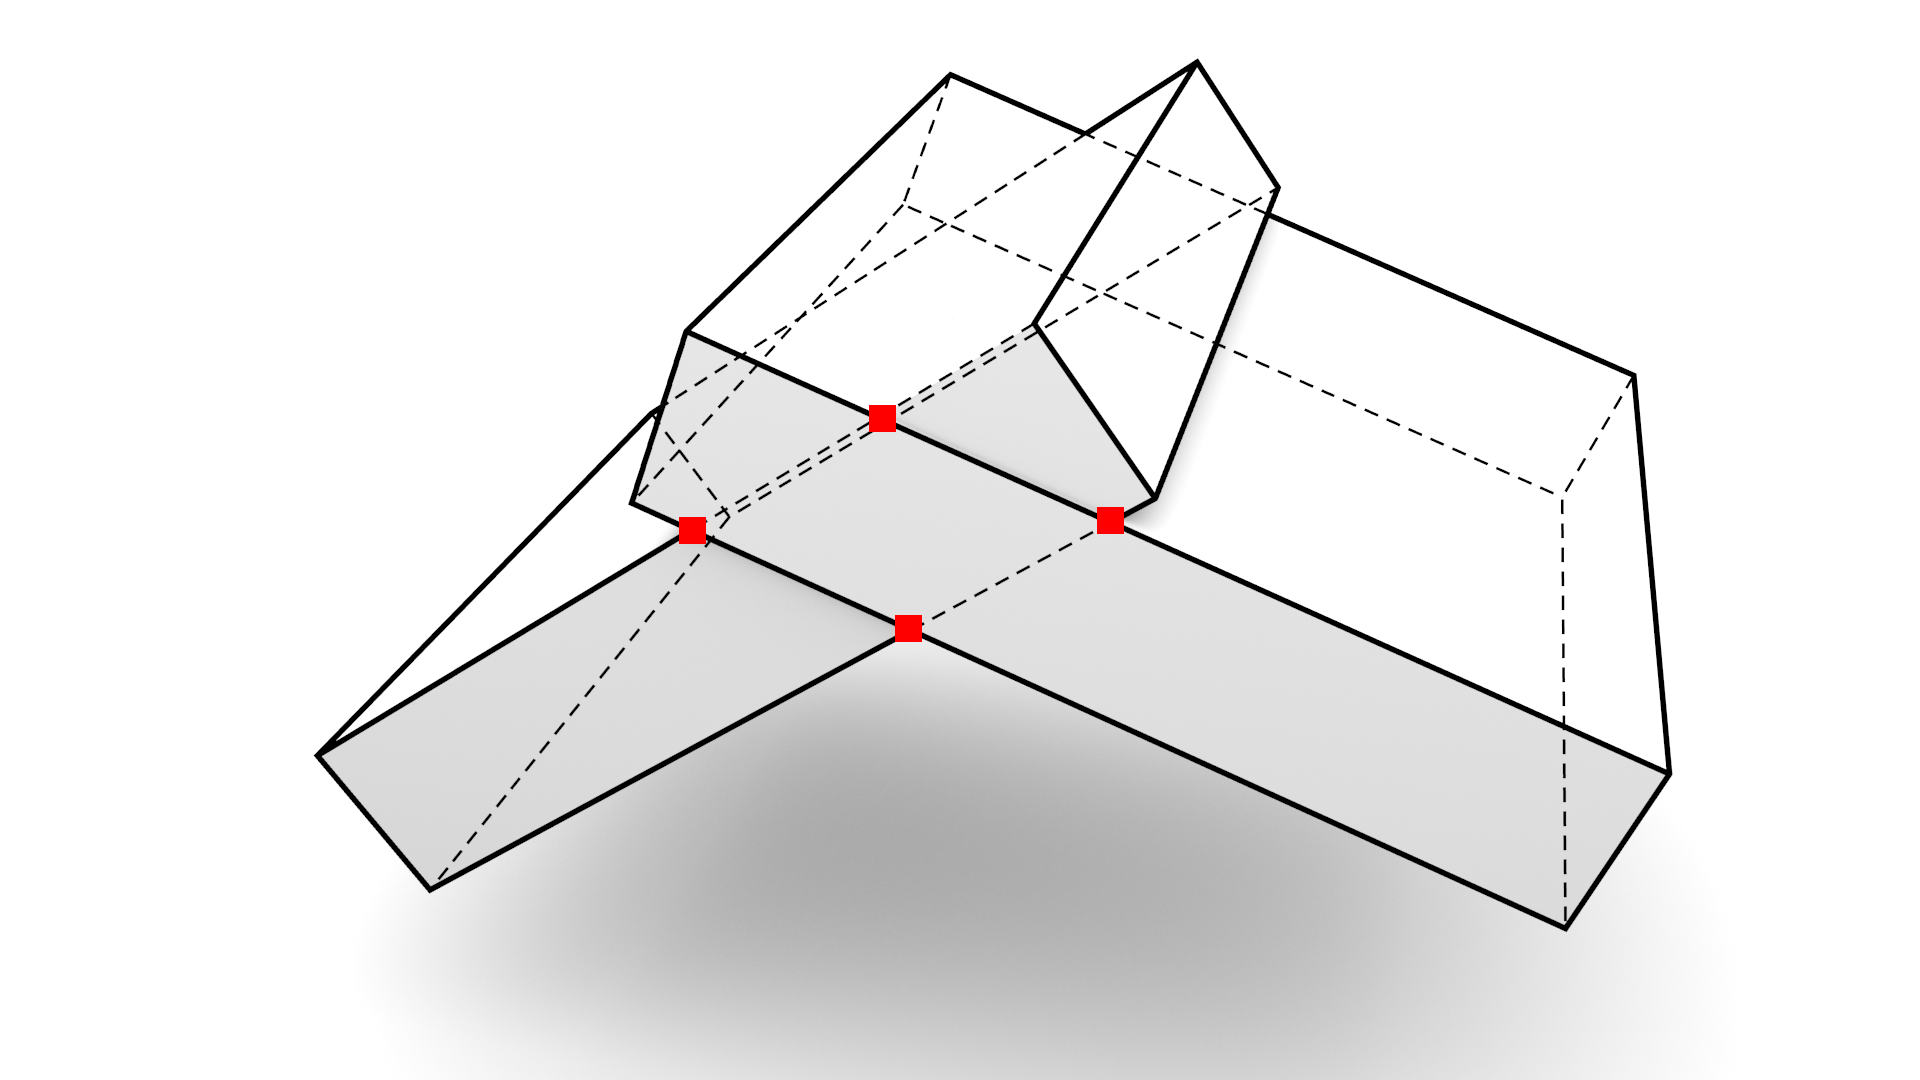
\includegraphics[width=\columnwidth]{Images/Blocks_obtuse_overintersect.png}
\caption{In this case the angle between the plates is obtuse. If we just took the inner intersection here without first clipping of the plates there would be no space for joints. Additionally, none of the intersection lines marked here in red lie on an outer boundary point. Therefore they would all have been marked as main. }
\label{fig:obtuseAssumption}
\end{figure}
This is why we replaced this algorithm with the one from the previous section \hyperref[mainLine]{Main Lines}.

\subsection{Adjusting angles based on which sides of the plates touch}
Our previous version of finding a main line was supposed to yield one line. Based on this line the angle was calculated with the following procedure:\\ 
After the angle of the planes had been calculated we adjusted the angle in some cases dependent on the direction in which the normals were pointing. \\
We know which sides of the plates are enclosing the angle thanks to the previous main line calculation.\\
In order to find out in which cases the angle has to be adjusted we check for two properties.\\
First, there is the question which of the sides of the plates intersect. A plate is defined by a 2D-shape which is called main side. The other side which exists due to a specified thickness of the plate is called parallel side.\\
Additionally, we look at the direction of the normals. The direction is positive when it is directed from the main to the parallel side and negative otherwise.\\
For an angle to be in need to be adjusted the following conditions need to be satisfied.
\begin{itemize}
    \item The two plates touch with the same type of side 
    \item[] AND
    \item Their directions are both positive OR both negative
\end{itemize}
But as mentioned before all of these calculations are based on the assumption that the previous main line calculation only yielded one line.\\
In this case the previous algorithm fails which is why we developed a new approach for finding the correct angle as already explained in the section \hyperref[angleCalculation]{Angle Calculation}.

\section{Future work}
A few more things have to be accomplished to allow for a smooth conversion. 
\subsection{Multiple line segments per edge}
Currently, we only calculate one line per edge but as can be seen in figure \ref{fig:twoLineSegments} this is not enough. To solve this the line segments should be found and for each segment a new edge should be created to be handles seperately. 
\begin{figure}[!ht]
\centering
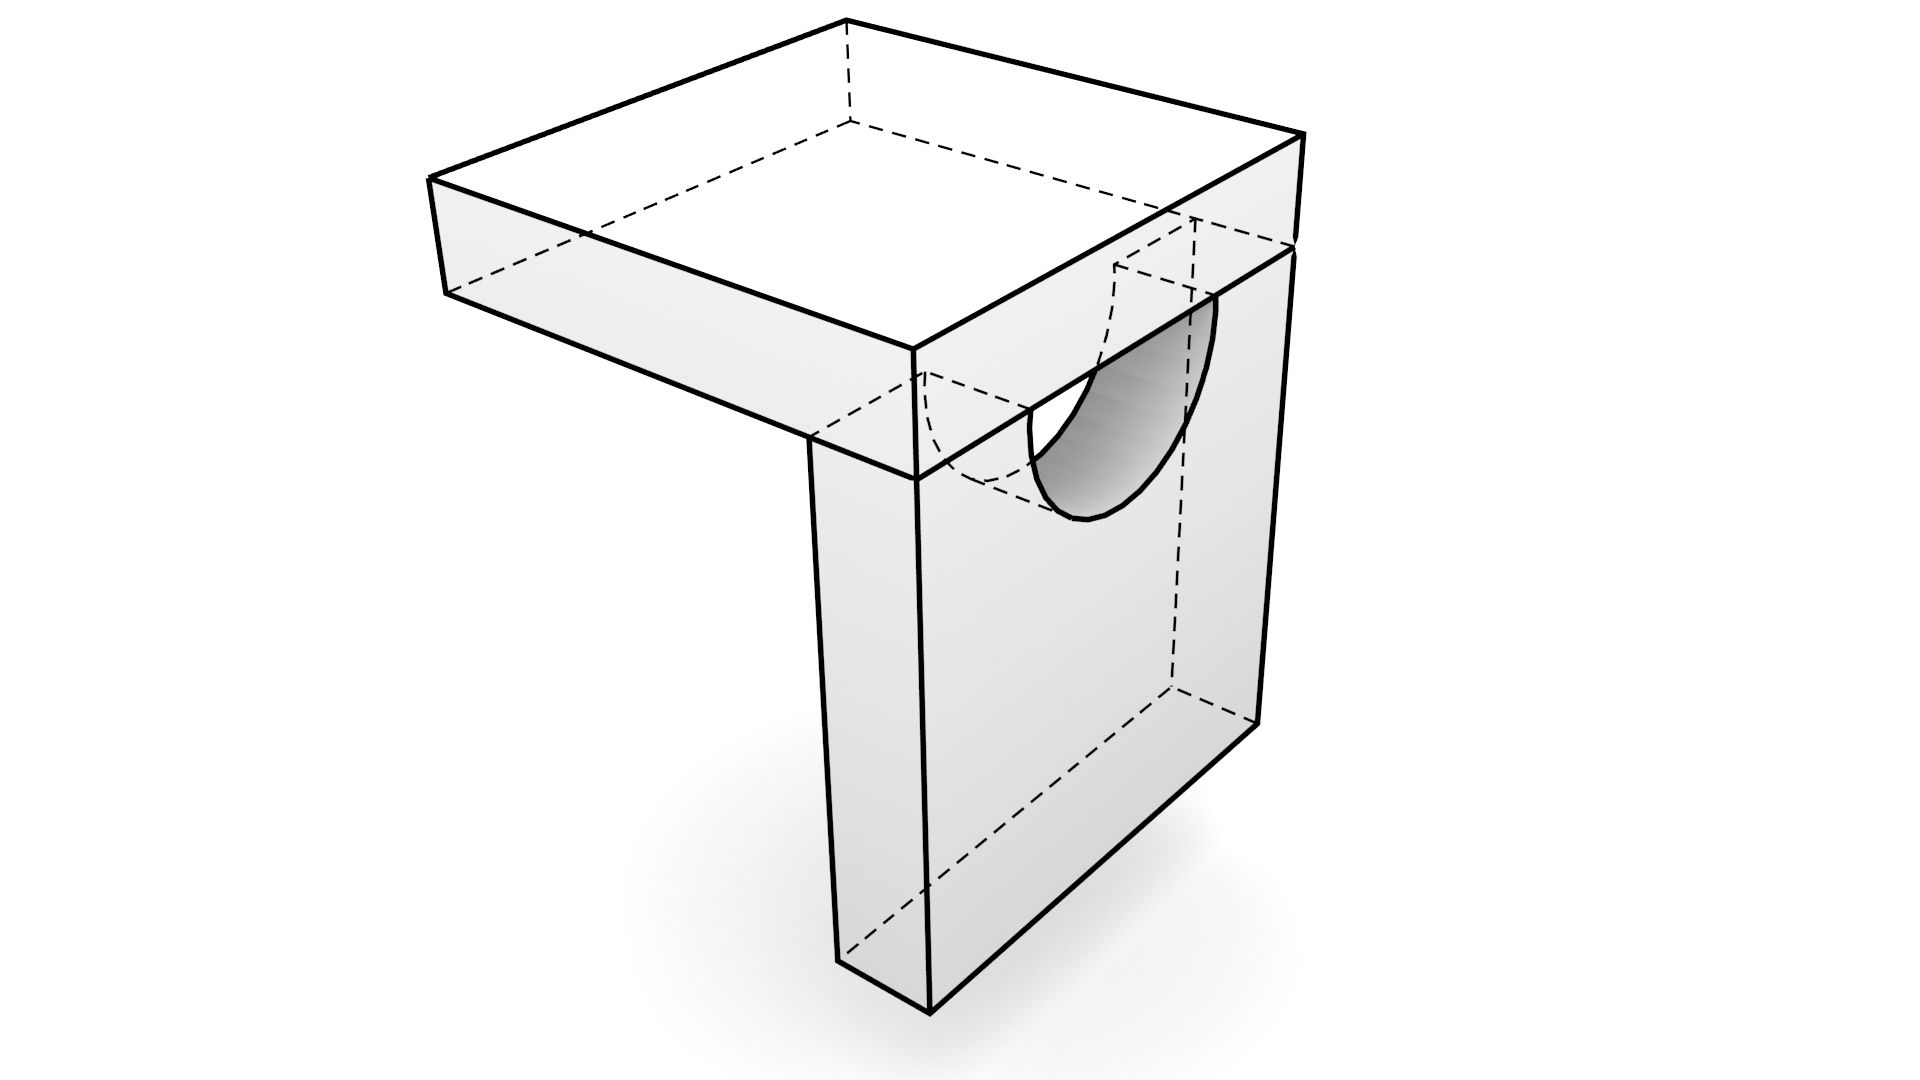
\includegraphics[width=\columnwidth]{Images/Blocks_two_contact(1).png}
\caption{Plate 2 touches Plate 1 twice. This should result in two edges and intersections which should be handled seperately.}
\label{fig:twoLineSegments}
\end{figure}

\subsection{Detect if the model is producible}
A very important information about the final converted model is if it can actually be build. A user may not only need assembly instructions on how to build the model when cut but also if it is possible to do so. There may be a conflict when plate \emph{a} needs to be added before plate \emph{b} but plate \emph{b} also needs to be put up before plate \emph{a}. This should never happen or at least be mentioned to the user.

\subsection{Rejoining broken up plates}
In the master thesis \cite{master-thesis} it was mentioned that plates can be split by another one standing perpendicular to it. This should result in a t-junction. Therefore the plate graph has to recognize those broken up plates and reunion them. The suggested solution is to group two plates together again when the following statements are true for three plates \emph{P1, P2, P3}:\\
    \begin{enumerate}
        \item the main sides of P1 and P2 are coplanar
        \item P1 and p2 have the same thickness
        \item P1 and P2 each have a shared edge with p3 that is parallel and which overlaps when projected onto each other
    \end{enumerate}
    In order to reunion such plates the following steps are necessary:
    \begin{enumerate}
        \item Iterate over all nodes and check if the current node has two or more neighbors. 
        \item Test if any of the neighbors are coplanar to each other. If so they are labeled as plates P1 and P2. Any other neighbor is labeled P3 or higher.
        \item Check if P1 and P2 have the same thickness. If not start over with the next node
        \item If they have the same thickness the intersection lines need to be checked to be parallel and overlaps between P1 and P3, and P2 and P3.
        \item When determined that P1 and P2 should actually be one plate which has been parted by P3 then they need to be unioned and marked for receiving a t-junction in the next step.
    \end{enumerate}

\end{document}